\documentclass[french, a4paper, 12pt]{report}
\usepackage[margin=2.5cm]{geometry}
\usepackage[utf8]{inputenc}
\usepackage[frenchb]{babel}
\usepackage[T1]{fontenc}
\usepackage{babel}
\usepackage{graphicx}
\usepackage{lettrine}
\usepackage{lmodern}
\usepackage{eso-pic}
\usepackage{tabularx}
\usepackage{titlesec}
\usepackage{colortbl}
\usepackage{xcolor}
\usepackage{setspace}
\usepackage{tikz}
\usepackage{hyperref}
\usepackage{stmaryrd}
\usepackage{subfig}
\usepackage{graphicx} 
\usepackage{caption}
\usepackage{mwe}
\usepackage{lipsum}
\usepackage{filecontents}
\usepackage{wrapfig}
\usepackage{url}
\usepackage{pdfpages}
\usepackage[shortlabels]{enumitem}
\usepackage[font=small,labelfont=bf]{caption}
\hypersetup{
    colorlinks=true,
%     linkcolor=blue,
    citecolor=black,
    filecolor=black,
    linkcolor=black,
    urlcolor=black
}


\definecolor{olivegreen}{rgb}{0,0.5,0}

\titleformat{\chapter}[hang]{\bf\LARGE}{\thechapter}{0pc}{ - }
\titleformat{\section}[hang]{\bf\Large}{\thesection}{0pc}{ - }
\titleformat{name=\chapter,numberless}[hang]{\bf\LARGE}{}{0pc}{}
\titleformat{name=\section,numberless}[hang]{\bf\Large}{\thesection}{0pc}{}
%%%%%%%%%%%%%%%%%%%%%%%%%%%%%%%%%%%%%%%%%%%%%%%%%%%%%
%%%%%%%%%%%%% PROJECT TITLE%%%%%%%%%%%%%%%%%%%%%%%%%

\title{Mémoire fin d'étude }


%%%%%%%%%%%%%%%%%%%%%%%%%%%%%%%%%%%%%%%%%%%%%%%%%%%%




\begin{document}
%%%%%%%%%%%%%%%%%%
%%% First page %%%
%%%%%%%%%%%%%%%%%%

\includepdf{images/cover2.pdf}
%\begin{titlepage}
%\begin{center}

%\begin{figure}[!htb]
%\minipage{0.25\textwidth}
 % 
\includegraphics[width=\linewidth]{images/parisNanterre-logo}
%\endminipage\hfill
%\minipage{0.2\textwidth}
 % 
\includegraphics[width=\linewidth]{images/logo_afia_2x.png}
%\endminipage\hfill
%\minipage{0.2\textwidth}%
%  
\includegraphics[width=\linewidth]{images/datategy.png}
%\endminipage
%\end{figure}
%\vspace{1cm}
%{\Large Mémoire de fin d'étude Master 2 MIAGE}\\[0.5cm]


% Title
%\rule{\linewidth}{0.5mm} \\[0.4cm]
%{ \huge \bfseries Quel est l'impact de la visualisation du Big Data sur les smart cities? \\[0.4cm] }
%\rule{\linewidth}{0.5mm} \\[1.5cm]
%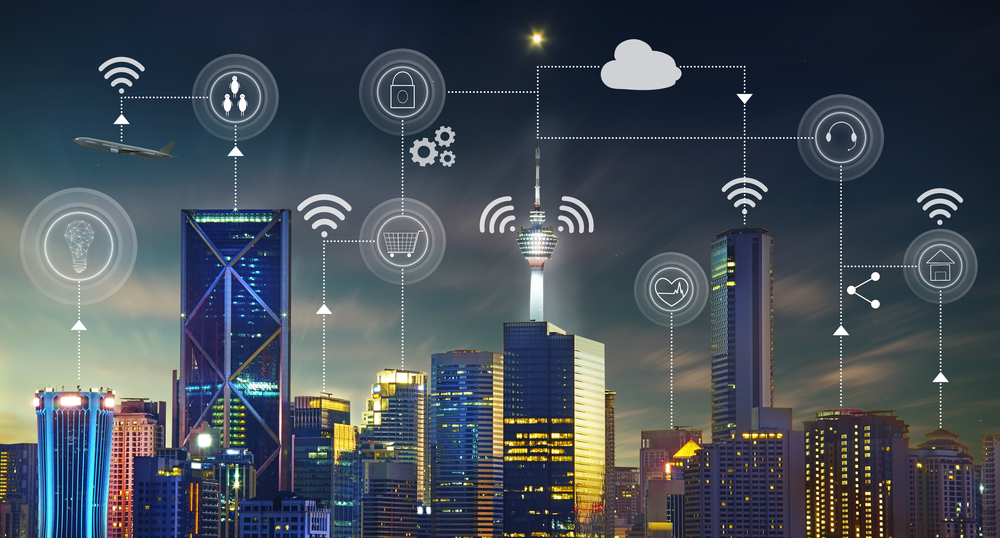
\includegraphics[width=1\textwidth]{images/Smart-City.jpg}\\[1cm]
% Author and supervisor
%\noindent
%\begin{minipage}{0.4\textwidth}
%  \begin{flushleft} \large
%    \emph{Étudiant :}\\
%    Hani \textsc{Abdulwahab}
%  \end{flushleft}
%\end{minipage}%
%\begin{minipage}{0.4\textwidth}
%  \begin{flushright} \large
%    \emph{Encadrants :} \\
%    Mme.~Sonia \textsc{GUEHIS}\\
%    M.~Mehdi \textsc{CHOUITEN }

%  \end{flushright}
%\end{minipage}
%
%\vfill

% Bottom of the page
%{\large Version 1.0 du\\ \today}

%\end{center}
%\end{titlepage}

\tableofcontents
%\listoffigures
\chapter*{Remerciements}
% Pour leur soutien, leur disponibilité et leur écoute tout au long de ce master MIAGE, je souhaite tout d'abord remercier Monsieur le professeur POIZAT, Monsieur le professeur GUYON et Madame CHAU, chargée d’insertion professionnelle. \\

% Pour m’avoir accordé sa confiance pour la réalisation de ce projet intéressant, je tenais à remercier Madame GUEHIS, responsable de mon stage.\\

% Pour m’avoir accompagné, conseillé et formé tout au long de ce stage, je tenais à remercier Monsieur VILLECROZE, encadrant mon stage.\\

% Pour l’aide technique, et les réponses à mes interrogations, j’adresse aussi mes remerciements à Monsieur DÉCOMBAS, ainsi que Monsieur CAPRA.\\

% Pour leur aide, les informations sur les stages et les offres, je tiens à remercier également toute l'équipe administrative du master MIAGE. \\

% Mes plus profonds remerciements vont à mes parents. Tout au long de mon cursus, ils m’ont toujours soutenu, encouragé et aidé, malgré la distance qui nous éloigne à présent. Je remercie en particulier mon cousin le Docteur Alain ABDULWAHAB et sa famille, pour m’avoir soutenu dans mes efforts depuis mon arrivée en France.  \\

% Je remercie tous mes plus proches amis, en ayant une pensée pour Nicolas ROUGE à qui je souhaite réussite et bonheur. \\

% Plus personnellement, je remercie ma bien-aimée, Zuleyha KABA, pour son soutien infini, son écoute et surtout son amour qui m’a été essentiel durant ces années. 
\chapter*{Introduction}
\addcontentsline{toc}{chapter}{Introduction}
Une ville intelligente idéale est une ville où l’on peut mener une vie saine et agréable. En tant qu’organisme vivant, une ville intelligente vérifie ses fonctions vitales, s’ajuste et se maintient saine, minimisant ainsi les inconvénients de l’urbanisation, loin des embouteillages, des pénuries de logements, des concentrations malsaines de poussière fine, des centres-villes surpeuplés, des structures sociales en ruine et du bruit.
L'expansion du Big Data et l'évolution des technologies de l'Internet des objets (IoT) ont joué un rôle important dans la faisabilité des initiatives de ville intelligente. Les mégadonnées offrent aux villes la possibilité d’obtenir des informations précieuses à partir d’un grand nombre de données recueillies auprès de diverses sources. L’Internet des objets permet l’intégration de capteurs, d’identification par radiofréquence et de Bluetooth dans un environnement réel utilisant des services hautement interconnectés. La combinaison de l'IoT  et du Big Data est un domaine de recherche inexploré qui a apporté de nouveaux défis intéressants pour atteindre l'objectif des futures villes intelligentes. Ces nouveaux défis se concentrent principalement sur des problèmes liés au business et à la technologie qui permettent aux villes d’actualiser la vision, les principes et les exigences des applications des villes intelligentes en réalisant les principales caractéristiques de l’environnement intelligent. Les smart cities sont le futur des grandes villes et les entreprises doivent décider de comment gérer les données et comment permettre à ses parties prenantes de prendre des décisions. Les données sont toujours plus nombreuses, plus complexes, plus variées et donc plus volumineuses, et plus particulièrement dans le cas des Smart Cities. Comment les analyser et en tirer profit pour prendre la meilleure décision au sein d’une entreprise afin de stimuler sa croissance ? \\

Actuellement, le contexte des villes modernes souhaitant devenir des villes intelligentes met en valeur la visualisation comme moyen d’analyse des données. La visualisation de données est la présentation de données dans un format graphique. Elle permet aux décideurs de voir les analyses présentées de manière visuelle, afin de pouvoir comprendre mieux et d’identifier de nouveaux modèles. Pour la business intelligence, la visualisation des données est très utile. Au lieu de parcourir un rapport comportant des centaines de lignes, un utilisateur professionnel peut simplement consulter un graphique. Les villes intelligentes apparaissent comme une stratégie de gestion de la performance urbaine, où il est nécessaire de visualiser un grand nombre de paramètres, souvent en temps réel. Les exigences du Big Data, les volumes croissants, les formats et normes de qualité variables, présentent des défis pour la gestion, le stockage, la visualisation et l'analyse des données, telles que la Geo-Visualisation et la Visual Analytics des données géospatiales. \\
La visualisation des données est devenue un centre d'intérêt pour la recherche, les industries, les gouvernements et les autres organisations afin d’améliorer la mobilité, l'efficacité énergétique, la gestion des déchets et l'administration publique d'une ville intelligente. Cela aide à mieux comprendre le système urbain et permet le développement durable des villes futures en améliorant les interactions humaines avec les données géospatiales.\\

Dans le cadre de mon Master M2 MIAGE en alternance à l’Université Paris Nanterre, j’ai souhaité réaliser un mémoire intitulé “Quels sont les techniques et les outils de la visualisation du Big Data dans les smart cities? “ pour décrire et comparer les différentes techniques et outils du Big Data dans les villes intelligentes. En effet, mon expérience en tant que développeur web front-end chez l’entreprise Datategy m’a fait découvrir l’intérêt de la visualisation à travers plusieurs tâches de visualisation Big Data.\\

Dans un premier temps, la définition théorique de la ville intelligente sera présenté. Cette définition se veut être un idéal vers lequel la ville intelligente veut tendre. L’impact de l'évolution des smart cities sur les domaines de l’économie, de la gouvernance, de l’environnement, de la mobilité et de la démographie seront analysés. Puis, le rôle de la technologie dans les smart cities, comprenant les données numériques (Big Data) et l’Internet of Things (IoT), sera abordé. De plus, la visualisation du Big Data, ses défis ainsi que les techniques et les outils de visualisation de données seront présentés. 
Dans un second temps, la réalisation d’une étude comparative entre les différentes techniques et outils de visualisation de données dans un contexte Big Data et smart cities seront présentés dans le chapitre suivant.
Dans un troisième temps, un cas pratique “la visualisation du Big Data chez Datategy” sera présenté, avec une étude comparative sur les différentes bibliothèques JavaScript de la visualisation Big Data. Par la suite, un bilan professionnel et personnel sera présenté. 


\chapter{Smart city  et  visualisation du Big Data}
\section{Smart city}
\subsection{Définition de la ville intelligente}
\subsubsection{Historique:}
La croissance des villes depuis la révolution industrielle a atteint des niveaux sans précédent. 
%La division de la population des Etats-Unis a estimé qu'en 2016, 54,5\% de la population mondiale vivait dans des zones urbaines et qu'en 2050, ce nombre atteindrait 67\% \cite{0}. 
Cette croissance considérable de la population urbaine nécessitera d’importants développements d’infrastructures urbaines pour faire face à la demande de ses habitants. Il ne fait aucun doute que les villes sont des systèmes complexes et que la croissance urbaine rapide engendre des embouteillages, une pollution et une inégalité sociale croissante. Ceux-ci peuvent transformer la ville en un point de convergence de nombreux risques (économiques, démographiques, sociaux et environnementaux). Cela pourrait sérieusement dépasser leur capacité à fournir des services adéquats à leurs citoyens \cite{1}. Cependant, des villes bien gérées peuvent offrir de multiples avantages aux personnes qui y vivent car elles permettent de réaliser des économies d’échelle en partageant des commodités telles que les transports, les installations de sport et de divertissement, les services aux entreprises, le haut débit, etc.
Depuis les années 1990, les gouvernements et les chercheurs utilisent le terme « villes intelligentes » comme un label de mode ou pour aider certaines villes à se distinguer et à se promouvoir comme innovantes. Être une ville intelligente est une aspiration pour certaines villes qui ont élaboré des plans à long terme afin d’atteindre cet objectif \cite{2}.
\subsubsection{Définition:}
De nombreuses études ont tenté de définir le concept de ville intelligente, mais le défi reste difficile à relever. C’est un concept multidisciplinaire et il est difficile de définir le terme « intelligent ». Les premières tentatives de définition du concept ont été axées sur l'intelligence des technologies de l'information pour la gestion de diverses fonctions de la ville \cite{3}. 
Dernièrement, les études ont élargi leur champ d'action en incluant les résultats de la ville intelligente tels que la durabilité, la qualité de vie et les services aux citoyens.
L'évaluation du niveau d'intelligence des villes est également devenue importante pour les chercheurs et les responsables gouvernementaux. Ils ont développé des classements prenant en compte des variables telles que l'économie, les infrastructures, l'innovation, la qualité de vie, les transports, le développement urbain, etc.
Malgré la vaste littérature sur les villes intelligentes, il existe plus de trente définitions du terme. Ils abordent des aspects différents, mais pertinents, notamment la construction de ces villes. 
Il ne fait aucun doute qu'une ville intelligente est un concept multidisciplinaire qui englobe non seulement son infrastructure informatique, mais également sa capacité à gérer les informations et les ressources pour améliorer la qualité de vie de ses habitants. L'utilisation de la technologie de l'information est considérée comme un facteur clé de l'intelligence d'une ville, car elle peut détecter, surveiller, contrôler et communiquer la plupart des services de la ville tels que les transports, l'électricité, le contrôle de l'environnement, la lutte contre la criminalité, les urgences sociales, etc \cite{4}.

\subsection{Étapes pour la mise en œuvre de projets de ville intelligente}

La mise en œuvre réussie d'un projet de ville intelligente nécessite la mise au point d'un système numérique capable de gérer et de visualiser les données géospatiales dans un environnement convivial. Le système d'information géographique (SIG) offre des fonctionnalités avancées et convivial pour les projets de ville intelligente.
Le concept de « ville intelligente » vise à développer un système complet qui utilise des données géospatiales pour améliorer la compréhension des systèmes urbains complexes et pour améliorer l’efficacité et la sécurité de ces systèmes. 
Ces données géospatiales concernent :
\begin{itemize}
\item \textbf{} L’environnement urbain construit tel que les infrastructures, les bâtiments et les espaces publics.
\item \textbf{} L’environnement naturel tel que la biodiversité, les espaces verts, la qualité de l’air, le sol et l’eau.
\item \textbf{} Les services urbains tels que les transports, les déchets municipaux, l’eau, l’énergie, la santé et l’éducation. 
\end{itemize} 
Le concept de ville intelligente vise également à transformer la gestion des villes «en silo» en un système «partagé» impliquant les acteurs urbains dans la conception, la réalisation et l’évaluation de projets urbains.
\begin{figure}[!ht]
    \centering
    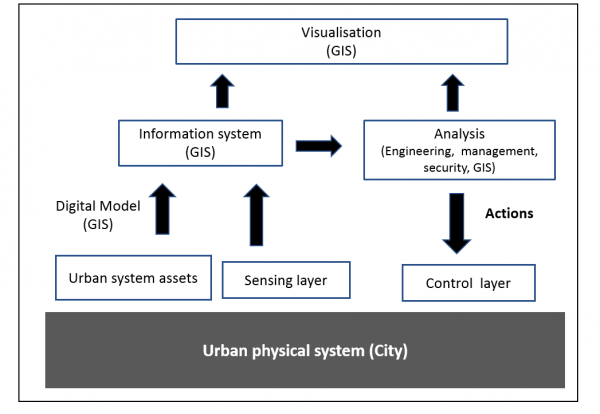
\includegraphics[height=8cm]{images/Steps.png}
    \caption{Étapes pour la mise en œuvre d’un projets de ville intelligente}
    \label{fig:2.1}
\end{figure}
Figure~\ref{fig:2.1} inclut la construction du modèle numérique urbain, la collecte de données à l'aide de la couche de détection, puis l'analyse des données, la visualisation interactive des données et le contrôle du système. Le SIG joue un rôle dans ces étapes, comme décrit ci-dessous. 

\subsubsection{1. Construction du modèle de ville intelligente:}
La première étape de la mise en œuvre d’un projet de ville intelligente concerne la construction du modèle numérique urbain qui décrit les composants des environnements urbains et naturels construits. Le modèle numérique fournit pour chaque composant urbain la géolocalisation et les caractéristiques (attributs). Les SIG sont généralement utilisés pour la construction du modèle numérique de «composants horizontaux» urbains tels que les réseaux urbains, les installations de transport et l’environnement naturel, tandis que la modélisation des données du bâtiment (BIM) est utilisée pour la description de «composants verticaux» tels que les bâtiments. La combinaison des SIG et du BIM fournit un outil puissant pour la construction du modèle numérique urbain avec des données géoréférencées et la visualisation de ces données dans un environnement convivial.

\subsubsection{2. Couche de détection:}
La deuxième étape d’un projet de ville intelligente concerne la construction de la couche de détection qui transfère les données d’exploitation urbaine au système d’information de la ville intelligente. Cette couche comprend des capteurs utilisés pour la surveillance des réseaux et infrastructures urbains. Les données pourraient également être enrichies d'images, de vidéos et de fichiers audio, ce qui aboutirait à la construction de mégadonnées urbaines. Par exemple le système d'eau potable utilise des lecteurs de compteurs automatiques (AMR) pour enregistrer la consommation d'eau, des capteurs de pression pour enregistrer la pression de l'eau et des dispositifs de contrôle de la qualité de l'eau permettant de suivre la qualité de l'eau (turbidité, pH, chlore, conductivité). Le système de drainage utilise des capteurs pour surveiller le niveau et le débit d'eau, la qualité de l'eau (turbidité, température, pH, etc.) et le matériel de pompage. Il permet une détection précoce des inondations et des défauts dans les équipements de pompage. Le réseau électrique utilise des capteurs pour mesurer la tension électrique, le courant et la fréquence. Il permet une détection précoce des défauts du réseau électrique. Le système de chauffage urbain est surveillé par des capteurs pour enregistrer la température, la pression et le débit du fluide, ainsi que l'état de la vanne. Il permet la détection précoce des pannes et l'amélioration des performances du système. Le SIG offre la possibilité de visualiser le système de surveillance ainsi que les caractéristiques et l’état des capteurs. Il offre également la possibilité de visualiser des données historiques et en temps réel sur des cartes SIG.
\subsubsection{3. L'analyse des données:}
La troisième étape de la mise en œuvre d'un projet de ville intelligente concerne le développement d'un environnement analytique, qui transforme les données en temps réel améliorant la sécurité, l'efficacité et la qualité des systèmes urbains. L'environnement analytique comprend des logiciels d'ingénierie, de gestion et de sécurité pour les systèmes urbains, ainsi que des outils numériques avancés tels que l'intelligence artificielle (IA). Dans les projets de ville intelligente, les SIG fournissent des outils pour (i) l’analyse de données géospatiales (traitement géométrique, modèles de grille), (ii) l’analyse spatio-temporelle, (iii) les statistiques spatiales (autocorrélation spatiale et modèle de régression), (iv) l’analyse de surface (analyse de la forme et du flux de surface, méthodes de maillage et d'interpolation) et (v) analyse de localisation (calcul du plus court chemin, localisation de l'installation).

\subsubsection{4. Visualisation interactive des données:}
La visualisation interactive des données permet aux utilisateurs d’interagir avec les composants de la ville intelligente et les parties prenantes (Skateholder) dans un environnement convivial. Les applications Web sont utilisées pour créer cet environnement interactif. L'utilisation de fenêtres contextuelles HTML permet aux utilisateurs d'accéder à du contenu Web, tel que des graphiques référencés par des URL. L'environnement graphique SIG interactif permet la visualisation de composants urbains et de cartes de capteurs. Les utilisateurs et les gestionnaires peuvent utiliser ces cartes pour accéder aux données statiques et dynamiques concernant les systèmes urbains ainsi que pour mettre à jour les données.

\subsubsection{5. Couche de contrôle}
L'analyse des données en temps réel et des données historiques donne lieu à des commandes pour une gestion optimale et sécurisée des systèmes urbains. Ces commandes sont transmises à la couche de contrôle, qui comprend différents dispositifs électroniques tels que des vannes intelligentes, des pompes, des moteurs, des commutateurs, des disjoncteurs et des serrures. Le système SIG permet une visualisation en temps réel de ces appareils ainsi que de leur statut. Il pourrait également visualiser les erreurs dans la commande de l'appareil.
%%%%%%%%%%%%%%%%%%%%%%%%%%%%%%%%%%%%%%%%%%%%%%%%%%%%%%%%%%%%%%%%%%%%%%%
\subsection{Avantages et opportunités}
Les avantages d’une ville intelligente sont notamment les suivants :
\begin{itemize}
\item \textbf{}Mise en place d’une gestion intelligente des infrastructures et des ressources naturelles.
\item \textbf{}Utilisation efficace des ressources avec les systèmes technologiques tels que la planification des ressources d'entreprise (ERP) et le système d'information géographique (SIG).
\item \textbf{}Meilleure qualité de vie pour les citoyens grâce à des services plus rapides, moins coûteux en temps et en énergie, à une meilleure planification des espaces et des lieux de vie et de travail, à des transports plus efficaces et à la disponibilité des informations concernant la ville pour les citoyens. 
\item \textbf{}Niveaux plus élevés de transparence et d’ouverture grâce au partage des données et des ressources, la transparence de l'information pour toutes les personnes impliquées encourage la collaboration et la communication entre entités et la création de plus de services et d'applications améliorant davantage la ville intelligente.
\end{itemize}
%%%%%%%%%%%%%%%%%%%%%%%%%%%%%%%%%%%%%%%%%%%%%%%%%%%%%%%%%%%%%%%%%%%%%%%
\section{Le rôle de la technologie dans les smart cities}
\subsection{Les données numériques (Big Data) }
Les applications Big Data peuvent potentiellement servir de nombreux secteurs dans une ville intelligente. Elles aident à fournir de meilleures expériences client et de meilleurs services, ce qui aident les entreprises à améliorer leurs performances. Améliorer les soins de santé en améliorant les services de soins préventifs, les outils de diagnostic et de traitement, la gestion des dossiers de santé et les soins aux patients. Les systèmes de transport peuvent grandement tirer parti des données volumineuses pour optimiser les itinéraires et les horaires, répondre aux demandes variées et être plus respectueux de l'environnement \cite{5}.
Le déploiement d’applications Big Data nécessite la mise en place d’une bonne infrastructure de technologies de l’information et de la communication (TIC). Les TIC soutiennent les villes intelligentes car elles apportent des solutions utiles, ainsi que des solutions uniques qui ne seraient peut-être pas possibles sans elles.
L’adoption de solutions TIC, Cloud et Big Data aide à résoudre de nombreux problèmes, tels que la fourniture des outils de stockage et d’analyse. En outre, cela aide à atteindre le stade de l'innovation et encourage la collaboration et la communication entre les différentes entités d'une ville intelligente.
Il existe de nombreux exemples d'applications Big Data servant les villes intelligentes telles que:
\begin{itemize}
\item \textbf{Education intelligente \cite{6}} : les TIC offrent une solution pour améliorer l'efficience, l'efficacité et la productivité des processus éducatifs grâce à des services éducatifs intelligents et flexibles permettant une meilleure utilisation de l'information, un contrôle et une évaluation améliorés, un soutien accru à l'apprentissage pour tous et tout au long de la vie. Les applications pédagogiques intelligentes impliquent les utilisateurs dans des environnements d’apprentissage actifs leur permettant de s’adapter aux changements rapides de la société et de l’environnement. Les mégadonnées dans l'éducation sont générées principalement par la collecte de données sur des personnes (par exemple des élèves, des enseignants, des parents, des administrateurs et d'autres personnels de soutien), des infrastructures (par exemple des écoles, des bibliothèques, des installations informatiques, des lieux d'enseignement, des musées et des universités) et des informations (cours, livres, examens, notes, enquêtes économiques, évaluations, rapports, etc). 
\item \textbf{Feux de circulation intelligents \cite{7}} : l’un des principaux aspects des villes intelligentes est un bon contrôle de la circulation dans la ville, ce qui améliore les systèmes de transport et les déplacements des citoyens ainsi que la structure générale du trafic des villes. L'utilisation de feux de signalisation intelligents et de signaux est l'une des techniques les plus importantes que les villes intelligentes utilisent pour faire face aux volumes de trafic et aux encombrements élevés. Les feux de signalisation intelligents et les signaux doivent être interconnectés sur les réseaux routiers pour offrir plus d'informations sur les schémas de trafic. Chaque capteur détecte un paramètre différent du flux de trafic (par exemple, la vitesse des voitures, la densité du trafic, le temps d'attente aux feux, les embouteillages, etc.). Le système prend des décisions en fonction des valeurs de ces paramètres et donne les instructions appropriées aux voyants et aux signaux. 
\item \textbf{Réseaux électriques intelligents :} appelés aussi Smart grids. Ce sont les réseaux électriques publics utilisent des télécommandes informatiques avec une technologie de communication bidirectionnelle entre les producteurs d'électricité et les consommateurs afin d'accroître l'efficacité et la fiabilité du réseau grâce à l'auto-surveillance et à la rétroaction du système. Cela implique de placer des capteurs et des compteurs intelligents sur les systèmes de production, de transmission et de distribution en plus des points d'accès des consommateurs pour obtenir des données granulaires en temps quasi réel sur la production, la consommation et les défauts actuels. Le traitement des données collectées, considérées comme une analyse de données volumineuses, en temps réel permet de renvoyer certaines informations de contrôle afin d'améliorer les performances globales du système d'alimentation électrique.
Cela permet la mise en oeuvre des modèles de tarification dynamiques pour la consommation d'énergie, d’éviter les pannes d’électricité potentielles dues à la forte demande des consommateurs et peut fournir aux consommateurs des informations en temps quasi réel sur leur consommation d'énergie et de faire fonctionner leurs appareils pendant les périodes de tarification plus basse. 

\end{itemize}


\subsection{l’Internet des Objets IdO}
Plus connu sous son sigle anglais IoT (Internet of Things) est la matérialisation d’Internet dans le monde réel qui offre une connectivité avancée des appareils intelligents, des appareils portables, des appareils et des services domestiques intelligents, des appareils médicaux, des véhicules connectés, des divertissements intelligents, des bâtiments intelligents et d’autres éléments reliés à un réseau d’Internet physique par une puce électronique, un capteur, une connectivité réseau leur permettant de communiquer entre eux, de collecter et d’échanger des données \cite{8}.
L'IoT fournit le corps de périphériques en communication. Un écosystème IoT se compose d’appareils intelligents activés sur le Web qui utilisent des processeurs, des capteurs et du matériel de communication intégrés pour collecter, envoyer et exploiter les données acquises dans leurs environnements. 
Les périphériques IoT partagent les données des capteurs qu'ils collectent en se connectant à une passerelle IoT ou à un autre périphérique, où les données sont envoyées au cloud pour être analysées ou sont analysées localement. Parfois, ces appareils communiquent avec d’autres appareils apparentés et agissent en fonction des informations qu’ils obtiennent les uns des autres. Les appareils effectuent la majeure partie du travail sans intervention humaine, bien que les utilisateurs puissent interagir avec eux, par exemple pour les configurer, leur donner des instructions ou accéder aux données.

Les protocoles de connectivité, de mise en réseau et de communication utilisés avec ces périphériques Web dépendent largement des applications IoT spécifiques déployées.

L'IoT offre de nombreux avantages aux organisations, leur permettant de :
\begin{itemize}
\item \textbf{}Surveiller leurs processus d'affaires globaux. 
\item \textbf{}Améliorer l'expérience client.
\item \textbf{}Gagner du temps et de l'argent. 
\item \textbf{}Améliorer la productivité des employés. 
\item \textbf{}Intégrer et adapter les modèles d'entreprise. 
\item \textbf{}Prendre de meilleures décisions d'affaires. 
\item \textbf{}Générer plus de revenus.
\end{itemize}
Il est important de comprendre que l’IoT ne fait pas référence à une seule technologie. C’est un concept englobant plusieurs techniques en même temps. Il faut donc penser à plusieurs systèmes à la fois quand on parle de cette notion.\\
Voici des exemples des différents systèmes impliqués dans l’IoT \cite{8}:
\begin{itemize}
\item \textbf{Identification :} Authentification de chaque objet et récolte des informations qu’il a emmagasiné.
\item \textbf{Capteur :} Collecte de données dans le but d’améliorer les capacités de l’appareil.
\item \textbf{Intégration : } Intégration de système pour une diffusion interne des données.
\item \textbf{Traitement d’informations :}  Accumulation de données et leur analyse dans le but de prendre une décision ou entreprendre un projet spécifique.
\item \textbf{Réseau :} Émission de données en ligne et dans le monde réel.
\end{itemize}

L'IoT encourage les entreprises à repenser leur façon d'aborder leurs activités, leurs industries et leurs marchés et leur donne les outils nécessaires pour améliorer leurs stratégies commerciales.
% \begin{figure}[!ht]
%     \centering
%     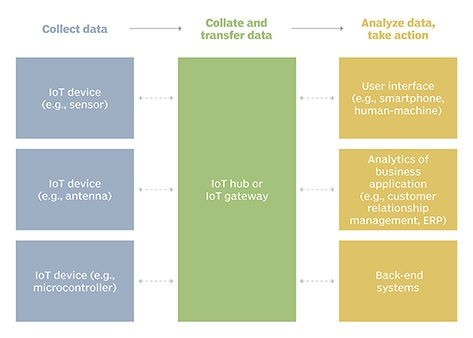
\includegraphics[height=9cm]{images/iot_system.jpg}
%     \scriptsize{source :\url{https://internetofthingsagenda.techtarget.com/}}
%     \caption{Exemple d'un systéme IoT}
%     \label{fig:1.2}
% \end{figure}
%%%%%%%%%%%%%%%%%%%%%%%%%%%%%%%%%%%%%%%%%%%%%%%%%%%%%%%%%%%%%%%%%%%%%%%
\subsection{Applications de Big Data et d'IoT dans les villes intelligentes}
L'application des technologies Big Data à la ville intelligente permet un stockage et un traitement efficaces des données afin de produire des informations susceptibles d'améliorer différents services de la ville intelligente. En outre, le Big Data aide les décideurs à planifier toute expansion des services et des ressources de la ville intelligente \cite{9}.Voici différentes applications de la ville intelligente:

\begin{enumerate}[a.] 
\item \textbf{Smart gouvernance :} soutient l'intégration et la collaboration de différentes agences gouvernementales et combine ou rationalise leurs processus. Cela se traduit par des opérations plus efficaces, un meilleur traitement des données partagées, une gestion et une application plus stricte de la réglementation.
Elle améliore les décisions commerciales grâce au support d'analyse Big Data. En recherchant le comportement et la croissance économique d’une entreprise en plus de ses concurrents et des conditions environnementales, les prises de décisions sont plus appropriées et plus efficaces en matière d’emploi, de production et de stratégies de localisation.
Elle permet la publication de nouvelles politiques au profit des propriétaires de données (citoyens) et des producteurs (agences gouvernementales). Les agences gouvernementales aident à développer la qualité des données, tandis que les citoyens montrent comment ils peuvent utiliser les données et les transférer vers de nouvelles connaissances afin d'améliorer la qualité des services publics.
Elle aident les gouvernements à se concentrer sur les préoccupations des citoyens en matière de santé et de protection sociale, de logement, d’éducation, de police et autres.\\

\item \textbf{Smart environnement :} fournit des informations météorologiques qui permettront d’améliorer l’agriculture du pays, de mieux informer la population sur les conditions potentiellement dangereuses et de mieux gérer l’utilisation de l’énergie en fournissant des prévisions plus précises à la demande.\\

\item \textbf{Smart mobilité :} reconnaît les modèles de trafic en explorant les données en temps réel. 
Elle réduit les embouteillages sur les routes principales de la ville en prévoyant les conditions de circulation et en ajustant les contrôles de circulation. Grâce au Big Data, la ville intelligente peut réduire le trafic et les accidents en ouvrant de nouvelles routes, en améliorant l'infrastructure en fonction des données de congestion et en collectant des informations sur le parking et les routes alternatives.
Elle réduit les déchets de la chaîne d'approvisionnement en associant les livraisons et en optimisant les mouvements d'expédition.
Elle active la transmission en continu des données pour traiter et communiquer aux conducteurs les informations sur le trafic collectées via des capteurs, des feux de signalisation intelligents et des dispositifs embarqués via des smartphones ou d'autres dispositifs de communication.
Les mégadonnées peuvent être utilisées pour envoyer des informations en retour à des entités spécifiques afin qu’elles prennent des mesures visant à atténuer ou à résoudre un problème de trafic.\\

\item \textbf{Smart énergie:} facilite la prise de décision concernant les niveaux d'approvisionnement en électricité en adéquation avec la demande réelle des citoyens et dans toutes les conditions qui affectent.
Elle permet la prévision en temps quasi réel grâce à une analyse efficace des données volumineuses collectées.
Elle s’aligne sur les objectifs stratégiques (optimisation des ressources) par le biais de plans de tarification spécifiques compatibles avec les modèles d'approvisionnement, de demande et de production.\\

\item \textbf{Smart éducation:} optimise la recherche universitaire. Par exemple, l'astronome peut maintenant analyser un grand ensemble de données astronomiques en utilisant des ordinateurs puissants au lieu d'analyses manuelles. En analysant et en explorant des images numériques de haute qualité prises depuis l'espace, de nouvelles découvertes peuvent se produire sur le terrain. Cela s'applique à de nombreux domaines scientifiques et de recherche tels que les expériences médicales, les opérations de fabrication, les études environnementales et les analyses économiques et financières.
Le comportement et le jumelage mèneront à de nouvelles connaissances. De l'évaluation des diplômés aux attitudes en ligne, chaque élève génère un suivi de données unique. En analysant ces données, les établissements d’enseignement peuvent déterminer s’ils utilisent leurs ressources aux bons endroits et produisent les bons résultats.\\

\item \textbf{Smart sécurité :} fournit des cartes des zones géographiques détaillées sur le plan spatial et le plan temprel, permettant ainsi d’aider à déterminer facilement les changements qui pourraient survenir.
Elle aide à prévoir les changements environnementaux futurs ou les catastrophes naturelles telles que la détection des tremblements de terre, qui permettront de sauver des vies et d'économiser des ressources.\\
\end{enumerate}

\subsection{Les exigences des applications de ville intelligente}
Les applications de ville intelligente basées sur le Big Data doivent répondre à plusieurs exigences découlant de la nature particulière des besoins de la ville intelligente et des caractéristiques du Big Data. Certaines exigences sont technologiques, tandis que d’autres sont liées à la sensibilisation des citoyens et aux rôles des gouvernements.\\
\subsubsection{Gestion des données volumineuses : }
Le principal avantage des applications de ville intelligente est qu’elles génèrent de gros volumes de données dans divers formats et dans de nombreux secteurs tels que le trafic, l’énergie, l’éducation, la santé et la fabrication. Ces données sont générées et collectées de manière massive et régulière, offrant ainsi une vue en temps réel de ce qui se passe dans la ville à tout moment. Pour garantir une utilisation appropriée et utile de ces données dans les applications de ville intelligente, il est important de disposer d'outils de gestion des données volumineuses appropriés et efficaces. La gestion des données volumineuses comprend le développement et l'exécution d'architectures, de politiques, de pratiques et de procédures qui gèrent correctement l'ensemble du cycle de vie des données tout au long de son utilisation dans les applications de ville intelligente. Comme les données proviennent de sources différentes avec des formats différents, il est nécessaire de disposer de fonctionnalités avancées de gestion des données permettant de reconnaître les différents formats et sources de données, de structurer, de gérer, de classer et de contrôler tous ces types et structures. La gestion des données volumineuses pour les applications de ville intelligente doit également permettre une gestion évolutive de données volumineuses afin de prendre en charge les applications hors ligne, ainsi qu'un traitement à faible temps de latence pour servir efficacement les applications en temps réel.\\
\subsubsection{Plateformes de traitement de données volumineuses:}
Les applications Big Data pour les villes intelligentes doivent effectuer des analyses de données qui nécessitent généralement une capacité de traitement énorme. Cela conduit à la nécessité de disposer des plateformes matérielles et logicielles évolutives et fiables. Les plateformes logicielles pour les villes intelligentes doivent offrir des capacités de calcul hautes performances, être optimisées pour le matériel utilisé, être stables et fiables pour les différentes applications nécessitant des données en cours d'exécution, prendre en charge le traitement de flux, fournir des niveaux élevés de résilience aux pannes et soutenu par une équipe et un fournisseur bien formés et compétents. Il existe différentes plateformes logicielles d'analyse des données volumineuses, telles que Hadoop Mapreduce , HPCC, Stratosphere et IBM Infosphere Streams, qui fournissent le traitement de flux requis par les applications de données volumineuses en temps réel. Ces plateformes fonctionnent bien sur des systèmes en cluster capables de fournir une plateforme matérielle, puissante et évolutive pour répondre aux exigences des applications de données volumineuses. Les mégadonnées peuvent également être traitées sur le Cloud en utilisant à la fois une plateforme Big Data (PaaS) et une infrastructure IaaS.\\
\subsubsection{Infrastructure de réseau intelligent:}

La plupart des applications Big Data pour les villes intelligentes exigent des réseaux intelligents connectant leurs composants, y compris les équipements des résidents, tels que les voitures, les appareils intelligents et les téléphones intelligents. Ce réseau doit être capable de transférer efficacement les données collectées de leurs sources vers le lieu de collecte, de stockage et de traitement des données volumineuses, ainsi que de renvoyer les réponses aux différentes entités qui en ont besoin dans la ville intelligente. La prise en charge de la qualité de service (QoS) sur le réseau est extrêmement importante pour les applications Big Data en temps réel destinées aux villes intelligentes. \\
\subsubsection{Algorithmes avancés:}
Les algorithmes standards utilisés dans les applications classiques peuvent ne pas être suffisants ou efficaces pour gérer les applications de données volumineuses en raison de leurs exigences spécifiques et de la nécessité impérieuse d'un traitement à grande vitesse et à haut volume. Les applications de données volumineuses pour les villes intelligentes doivent mettre en œuvre des algorithmes avancés et plus sophistiqués pour traiter efficacement les données volumineuses. Certains de ces algorithmes doivent être conçus pour la prise en charge d'applications en temps réel, tandis que d'autres peuvent être conçus pour un traitement par lots ou hors ligne. Ces algorithmes doivent être optimisés pour gérer des volumes de données élevés, une grande variété de types de données, des contraintes de temps sur les processus de prise de décision et des composants distribués sur divers emplacements géographiques. De plus, ces algorithmes doivent fonctionner efficacement dans des environnements hétérogènes et être capables de gérer et de fonctionner dans des environnements hautement dynamiques.\\
\subsubsection{Sécurité et confidentialité:}
Étant donné que la plupart des données collectées et traitées dans les applications de ville intelligente contiennent une forme d’information confidentielle, il est important de veiller à ce que tous les composants de la technologie et des applications incluent et maintiennent des niveaux acceptables de mécanismes de sécurité et de confidentialité. Bien qu'une ville intelligente offre de nombreux avantages positifs à ses résidents, elle fait peser de nombreuses menaces sur leur sécurité, leur bien-être et leur vie privée en s'appuyant fortement sur leurs données. La possibilité d'accès illégal ou d'attaques malveillantes à de telles infrastructures peut entraîner des résultats catastrophiques pour l'infrastructure de la ville, ses entités gouvernementales et ses résidents. Les concepteurs et les développeurs d’applications Big Data doivent inclure les politiques et les procédures de sécurité et de confidentialité, dans la conception et la mise en œuvre de leurs applications. \\
\subsubsection{Sensibilisation des citoyens:}
Les citoyens doivent savoir utiliser correctement et en toute sécurité les solutions TIC pour une ville intelligente. Leur participation active au gain d'informations sur les différents problèmes rencontrés avec les applications de ville intelligente contribue à améliorer la qualité des données collectées et la performance des applications. Un autre aspect important de la sensibilisation des citoyens est leur connaissance et leur usage de bonnes pratiques en matière de sécurité et de protection de la vie privée. \\
\subsubsection{Rôle du gouvernement:}
Les entités gouvernantes des villes intelligentes doivent établir des principes directeurs d'ouverture, de transparence, de participation et de collaboration afin de contrôler les échanges et le flux de données volumineuses [14]. Les gouvernements jouent un rôle essentiel dans une ville intelligente. Le gouvernement doit revoir et réajuster les politiques en matière d'informations et de données, en fonction des besoins, en mettant l'accent sur la confidentialité, la réutilisation des données, la précision des données, l'accès aux données, leur archivage et leur conservation [14]. 
Pour prendre en charge efficacement les applications de données volumineuses, le gouvernement des villes intelligentes doit établir un équilibre entre les utilisations bénéfiques des données et les préoccupations des particuliers en matière de vie privée, en abordant certains des concepts fondamentaux des lois sur la vie privée.\\


\section{Visualisation du Big Data }
\subsection{Context}
Les villes cherchent à devenir intelligentes en connectant les systèmes isolés des organismes municipaux et en installant des capteurs intelligents. Les administrateurs de la ville cherchent à exploiter les informations tirées des données des capteurs de l'Internet des objets (IoT), de systèmes de positionnement global (GPS), de smartphones et d'ordinateurs. 80\% de ces données sont des données sombres, ce qui signifie que les données sont non structurées pour transmettre un sens en soi \cite{10}.
Il est important de visualiser les données traitées pour découvrir les modèles et pour décider les prochaines étapes. Dans le but de faire ce processus efficacement, il est extrêmement important que les décideurs puissent visualiser et interagir avec les données.
Cela signifie qu'il est possible de supprimer la dépendance sur des experts en données de la boucle, ce qui signifie aussi que la plateforme de visualisation de données doit être interactive pour interagir avec les données, donc les idées deviennent visuellement évidentes dans le processus de découverte.

\subsection{L’importance de la visualisation du Big Data}
La visualisation de données, qui exploite la puissance de la réalité virtuelle, de la réalité augmentée et de l’apprentissage automatique, est une plateforme idéale pour la visualisation de flux de données IoT. La visualisation naturelle basée sur les gestes est non seulement intuitive, mais elle est également capable de montrer des données spatiales et temporelles complexes sur la réplique virtuelle d’un environnement, par exemple le modèle Google Earth ou le prototype 3D d’une ville.
La nouvelle technologie nous libère des cages de données à écran plat bidimensionnelles et nous permet de pénétrer dans nos données elles-mêmes en nous aidant à découvrir des informations grâce à un moyen de corrélation visuelle simpliste mais très puissant. Il n’est pas difficile de prendre des décisions avec la visualisation des données.
Plusieurs avantages plus spécifiques méritent d’être pris en compte. Voici quelques-uns des avantages les plus précieux de la visualisation de données volumineuses :
\subsubsection{1. Traiter rapidement de grandes quantités de données:}
Avec autant d’informations saisies, organisées et analysées, il y a tout simplement trop de données brutes pour que l’esprit humain moyen puisse les traiter à un rythme raisonnable. La visualisation de données volumineuses supprime le long processus de compréhension des données et permet aux utilisateurs de digérer rapidement des quantités de données volumineux et complexes. Ceci est souvent accompli par l’utilisation de tableaux de bord interactifs, présentés visuellement.
\subsubsection{2. Accéder aux données importantes en temps réel:}
Dans le monde des affaires au rythme rapide, chaque seconde compte. Les entreprises qui doivent s’appuyer sur des méthodes plus traditionnelles pour rassembler et affiner une grande quantité de données se retrouvent souvent avec des informations obsolètes. D'autre part, les meilleurs outils de visualisation de données volumineuses fonctionnent en temps réel et mettent constamment à jour les informations présentées. Ainsi, chaque fois qu'un utilisateur a besoin d'y accéder, il dispose toujours des données les plus récentes.
\subsubsection{3. Voir les liens entre les processus métier et les performances:}
Même si peu de dirigeants nieraient le fait que les processus et les activités opérationnels quotidiens d’une organisation aient un impact direct sur les performances globales de l’entreprise, il peut être difficile de voir exactement comment ces activités affectent le succès de la société. Les outils de visualisation de données volumineuses résolvent ce problème en permettant aux dirigeants de découvrir visuellement les relations cachées qui relient les processus quotidiens aux performances de l'entreprise.
\subsubsection{4. Raconter une histoire à travers des données:}
L'esprit humain a tendance à préférer traiter les informations de manière linéaire, c'est-à-dire qu'il aime voir les causes, les effets et les résolutions alignés de manière à raconter une histoire. En présentant les données de manière centrée visuellement, la visualisation de données volumineuses donne à l’information quelque chose qui lui manque généralement : un sentiment de progression. Cela rend la compréhension plus facile et l’utilisation aussi à utiliser pour les utilisateurs.
\subsection{Les éléments déterminant le choix de visualisation du Big Data:}
La visualisation est la première étape pour donner du sens aux données. Pour transcrire et présenter de manière simple les corrélations de données, les analystes de données utilisent un large éventail de charts, de diagrammes et de cartes. Le choix de la bonne technique et de sa configuration est souvent le véritable enjeu pour rendre les données compréhensibles. Et inversement, l’utilisation de techniques erronées peut ne pas présenter tout le potentiel des données, voire les rendre non pertinentes. Les nombreux facteurs qui influencent les choix de visualisation des données sont :
\subsubsection{1. L’audience:}
Il est important d’ajuster la représentation des données au public cible. Par exemple, si ce sont des clients finaux qui parcourent leurs progrès dans une application de sport, la simplicité est de mise. Par contre, si les analyses de données sont destinées à des chercheurs ou à des décideurs expérimentés, il est nécessaire d’aller au-delà des simples graphiques.
Il faut décider les données que la visualisation affichera, quels sont ses objectifs et ce qu’elle peut éventuellement révéler. Chaque visualisation doit avoir un objectif clairement défini pour piloter sa création.
\subsubsection{2. Le contenu:}
Ce qu’il faut présenter est aussi important que celui à qui il faut le montrer. Il existe 4 méthodes de base pour aborder la visualisation de données:
- Relations: il indique les liens et l'impact mutuel entre des éléments spécifiques (tels que le niveau d'éducation et le revenu moyen). Le nuage de points (Scatter plot) est le meilleur choix dans ce cas.
- Timeframe: les graphiques linéaires conviennent parfaitement si l’objectif est de montrer comment un certain phénomène se développe au fil du temps.
- Composition: cette technique est développée pour révéler la structure d'une seule unité, en montrant ses éléments constitutifs. La méthode la plus simple consiste à utiliser un graphique à secteurs, mais s’il est nécessaire d’obtenir une visualisation des données plus précise, le graphique à barres horizontales empilées à 100\% ou un graphique en pente est un bon choix.
- Comparaisons: les diagrammes à barres sont habituellement utiliser pour  comparer deux valeurs ou plus.
\subsubsection{3. Le contexte: }
Il est possible d’utiliser différentes approches pour l'apparence des graphiques et par conséquent, il est nécessaire de les lire en fonction du contexte. Pour souligner un certain chiffre, par exemple une forte croissance des bénéfices par rapport aux années précédentes, il est possible d’utiliser les nuances d’une couleur et choisir celle qui est brillante pour l’élément le plus significatif du graphique. Au contraire, pour différencier les éléments, il est recommandé d’utiliser des couleurs contrastées.
\subsubsection{4. La dynamique:  }
Il existe différents types de données, chacune impliquant un taux de changement différent. Par exemple, les résultats financiers peuvent être mesurés tous les mois ou tous les ans, tandis que les séries chronologiques et les données de suivi changent constamment. Selon le type de changement, une représentation dynamique (steaming) ou une visualisation statique peuvent être envisagés.
\subsubsection{5. L’objectif:  }
L’objectif de la visualisation des données a également une influence considérable sur la manière dont elle est mise en œuvre. Afin d'effectuer une analyse complexe d'un système ou de combiner différents types de données pour une vue plus détaillée, les visualisations sont compilées dans des tableaux de bord avec des contrôles et des filtres. Cependant, les tableaux de bord ne sont pas nécessaires pour afficher un aperçu des données unique ou occasionnel.
\subsubsection{6. Les couleurs: }
Les couleurs choisies auront un impact important sur l'efficacité globale de modèle de visualisation de données. Il est important de maintenir la cohérence des couleurs dans les documents et le contraste.
7. Utiliser des cartes interactives
La visualisation de données peut devenir une source de contenu numérique précieux, ce qui nécessite l'ajout d'éléments interactifs à la présentation. Les cartes interactives jouent un rôle majeur à cet égard car elles permettent aux utilisateurs de s’engager et de ne rechercher que les informations dont ils ont réellement besoin.
Les cartes interactives permettent aux utilisateurs de parcourir le graphique, d'effectuer des zooms avant et arrière, d'identifier des éléments spéciaux au clic, d'obtenir une vue d'ensemble à 360 degrés et de nombreuses autres fonctionnalités intéressantes. La création de telles cartes est un processus très complexe, mais elle laissera certainement une bonne impression aux clients.


%%%%%%%%%%%%%%%%%%%%%%%%%%%%%%%%%%%%%%%%%%%%%%%%%%%%%%%%%%%%%%%%%%%%%%%%

\chapter{Les techniques et les approches de la visualisation du Big Data}
Donner un sens aux faits, aux chiffres et aux mesures est une forme d'art, l'art de la visualisation de données. Les scientifiques de diverses disciplines utilisent des techniques informatiques pour modéliser des événements complexes et visualiser des phénomènes qui ne peuvent pas être observés directement, tels que les conditions météorologiques, les conditions médicales ou les relations mathématiques.
\section{Les techniques de visualisation du Big Data}
La visualisation de données fournit une suite importante d’outils et de techniques permettant d’obtenir une compréhension qualitative. Dans cette section, les différentes techniques de base tels que les graphiques, les infographiques,  les cartographies et géo-visualisation seront présentés.
\subsection{Les graphiques:}
Il existe quatre catégories de graphiques de base, qui peuvent être utilisés pour présenter les données (Comparaison , Composition , Distribution et Relation).
\begin{figure}[!ht]
    \centering
    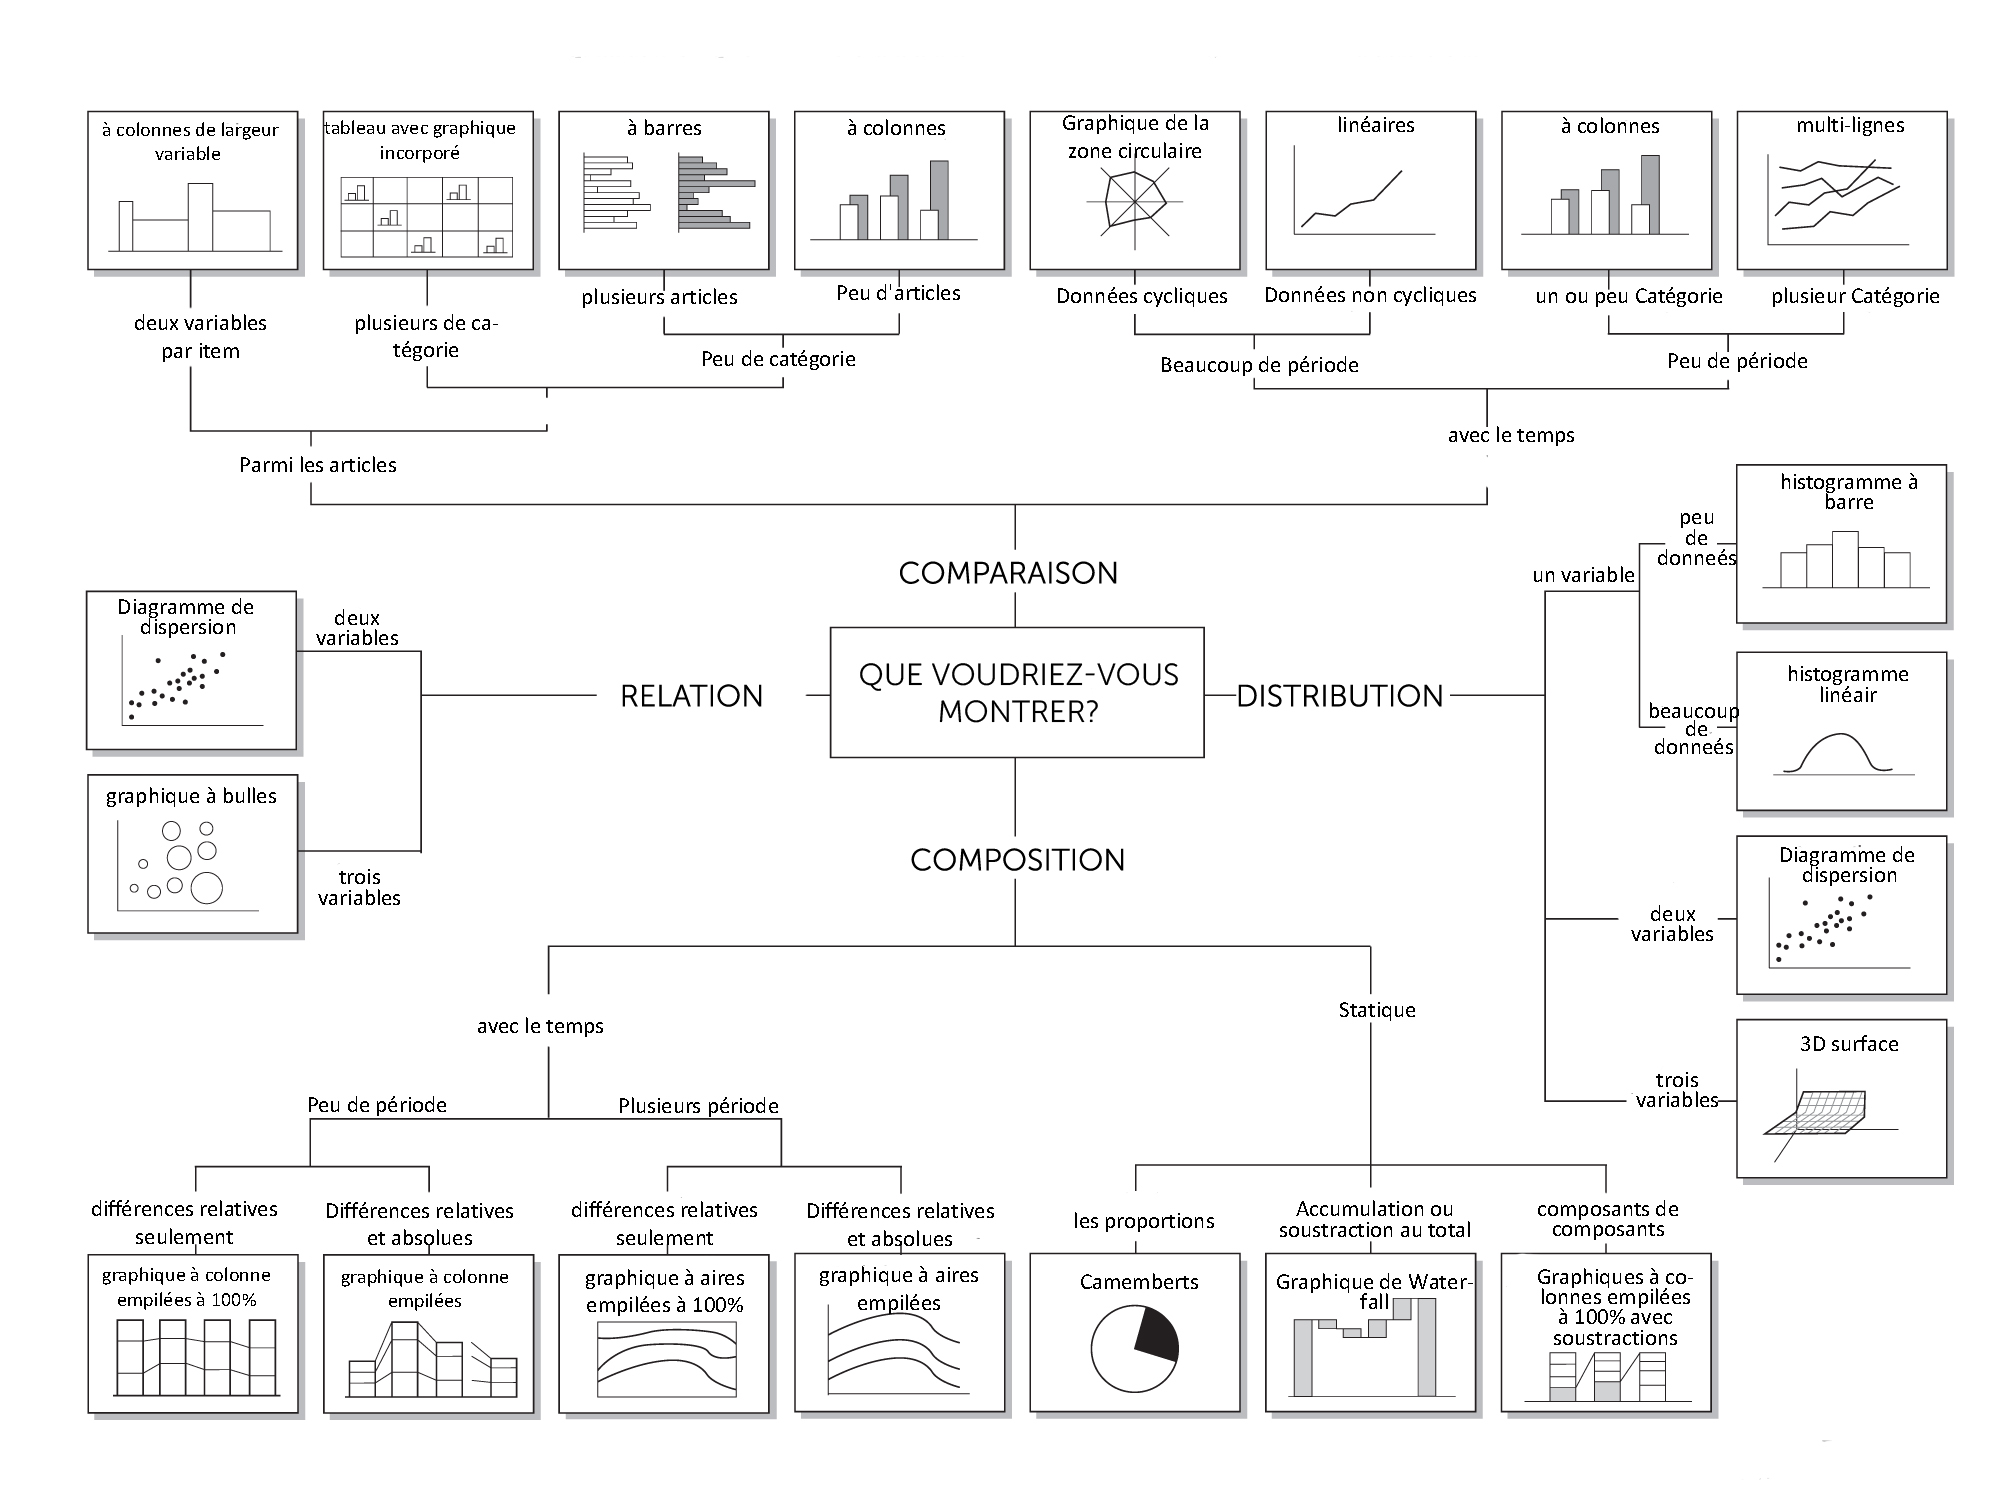
\includegraphics[height=8cm]{images/diagramme-de-charts.jpg}
    \caption{Le diagramme de sélection de graphique \footnotemark}
    \label{fig:2.1}
\end{figure}
\footnotetext{source : \url{https://eazybi.com/blog/data_visualization_and_chart_types/}}
 Le diagramme de sélection de graphique illustré à la figure ~\ref{fig:2.1}
, permet de choisir le bon graphique en fonction du type de données.
\subsubsection{1. Comparaison: }
Ces visualisations se rapportent au temps et à la taille des données. Les graphiques de comparaison sont utilisés pour comparer la magnitude des valeurs et peuvent être utilisés pour trouver facilement les valeurs les plus basses et les plus hautes dans les données. Les graphiques de comparaison peuvent être également utiliser pour comparer les valeurs actuelles par rapport aux valeurs anciennes afin de déterminer si les valeurs augmentent ou diminuent. Les questions les plus courantes sont «quels produits se vendent le mieux» et «comment nos ventes se comparent-elles à celles de l'année dernière».
Il n’existe pas un seul graphique à utiliser pour toutes les données synchronisées; certaines situations requièrent des graphiques linéaires tandis que d'autres nécessitent des graphiques à barres ou des graphiques en aires (pour les données cycliques).
Par exemple, pour un nombre moins élevé de catégories parmi les éléments, le  graphique à barres affiche mieux les différences entre les données que les camemberts. C’est la raison pour laquelle il est préférable d’utiliser un graphique à barres qu’un graphique à secteurs lorsqu'il est question de comparaison.
\subsubsection{2. Composition:}
Les graphiques de composition sont utilisés pour voir comment une partie se compare à la totalité et comment une valeur totale peut être divisée en plusieurs valeurs. Un graphique de composition montre la valeur relative, mais certains graphiques peuvent également être utilisés pour montrer la différence absolue. La différence est entre regarder le pourcentage du total et la valeur du total. Les questions communes sont «quelle part du marché nous avons dans une région» ou «en quels domaines notre budget est-il divisé».
Ces visualisations font référence à des ensembles de données qui évoluent dans le temps ou incluent des données statiques. Avec les données statiques, un diagramme à secteurs peut fonctionner.
\subsubsection{3. Relations : }
Les diagrammes de relations sont utilisés pour voir la relation entre les données et peuvent être utilisés pour trouver des corrélations, des valeurs aberrantes et des grappes de données. Les questions courantes sont les suivantes: «existe-t-il une corrélation entre les dépenses publicitaires et les ventes de nos produits» ou «comment les dépenses et les revenus varient-ils d’une région à l’autre et quel est l’écart»

\subsubsection{4. Distribution: }
Les graphiques de distribution sont utilisés pour voir comment les valeurs quantitatives sont réparties le long d'un axe, du plus bas au plus élevé. En examinant la forme des données, un utilisateur peut identifier des caractéristiques telles que la plage de valeurs, la tendance centrale, la forme et les valeurs aberrantes. Il peut être utilisé pour répondre à des questions telles que «nombre de clients par groupe d'âge» ou «combien de jours en retard ont nos paiements».
Pour illustrer mieux ce type de graphique, le graphique de nuages de points (Scatter plot) est illustré à la figure ~\ref{fig:2.2} et présenté ci-dessous :
\pagebreak

En affichant une variable dans chaque axe, il est possible de détecter une relation ou une corrélation entre les deux variables.
\begin{figure}[!htb]
\begin{minipage}{0.46\linewidth}
Différents types de corrélation peuvent être interprétés à travers les modèles affichés sur les diagrammes de dispersion. Il existe une corrélation positive (les valeurs augmentent ensemble), négative (une valeur diminue avec l’augmentation), nulle (pas de corrélation), linéaire, exponentiel et en forme de U. La force de la corrélation peut être déterminée par la proximité des points sur le graphique. Les points qui finissent loin du groupe général de points sont appelés points aberrants.
Des lignes ou des courbes sont ajustées dans le graphique pour faciliter l'analyse et sont dessinées aussi près que possible de tous les points. Ainsi, il est montré comment tous les points ont été condensés en une seule droite. Ceci est généralement connu sous le nom de Droite de meilleur ajustement et peut être utilisé pour effectuer des estimations par interpolation.
Les diagrammes de dispersion sont parfaits lorsqu’il est associé des données numériques et que l’objectif est de voir si une variable a un impact sur l'autre. Cependant, il est important de rappeler que la corrélation n'est pas une cause et qu'une autre variable inaperçue peut influer sur les résultats.
\end{minipage}\hfil
\begin{minipage}{0.35\linewidth}
    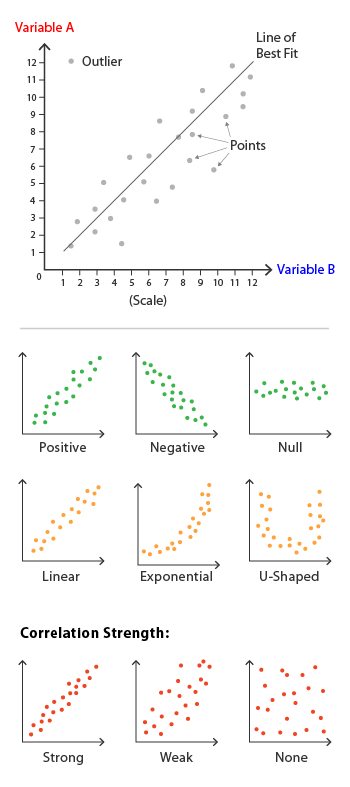
\includegraphics[height=13cm]{images/scatter-plot.png}
    \caption{\small Diagramme de dispersion \footnotemark}
 \label{fig:2.2}
\end{minipage}
\end{figure}
\footnotetext{source : \url{https://datavizcatalogue.com/methods/scatterplot.html}}
\subsection{Infographie}
Les infographies sont devenues un moyen de communication de masse; ils sont conçus pour atteindre un public plus large en simplifiant les sujets complexes et en les organisant dans un format facile à digérer, contrairement à d'autres types de visualisations. \\*
Une infographie (graphique d'information) est une représentation visuelle de l'information qui vise à rendre les données facilement compréhensibles au premier coup d'œil. Une infographie utilise au minimum le texte et peut constituer un outil puissant pour afficher des données, expliquer des concepts, simplifier les présentations, cartographier les relations, afficher les tendances et fournir des informations essentielles.Les infographies se présentent sous différentes formes. Ils sont classés en fonction de leur objectif, des types d’objets utilisés et du flux d’informations. 
\newpage
\begin{figure}[!ht]
    \centering
    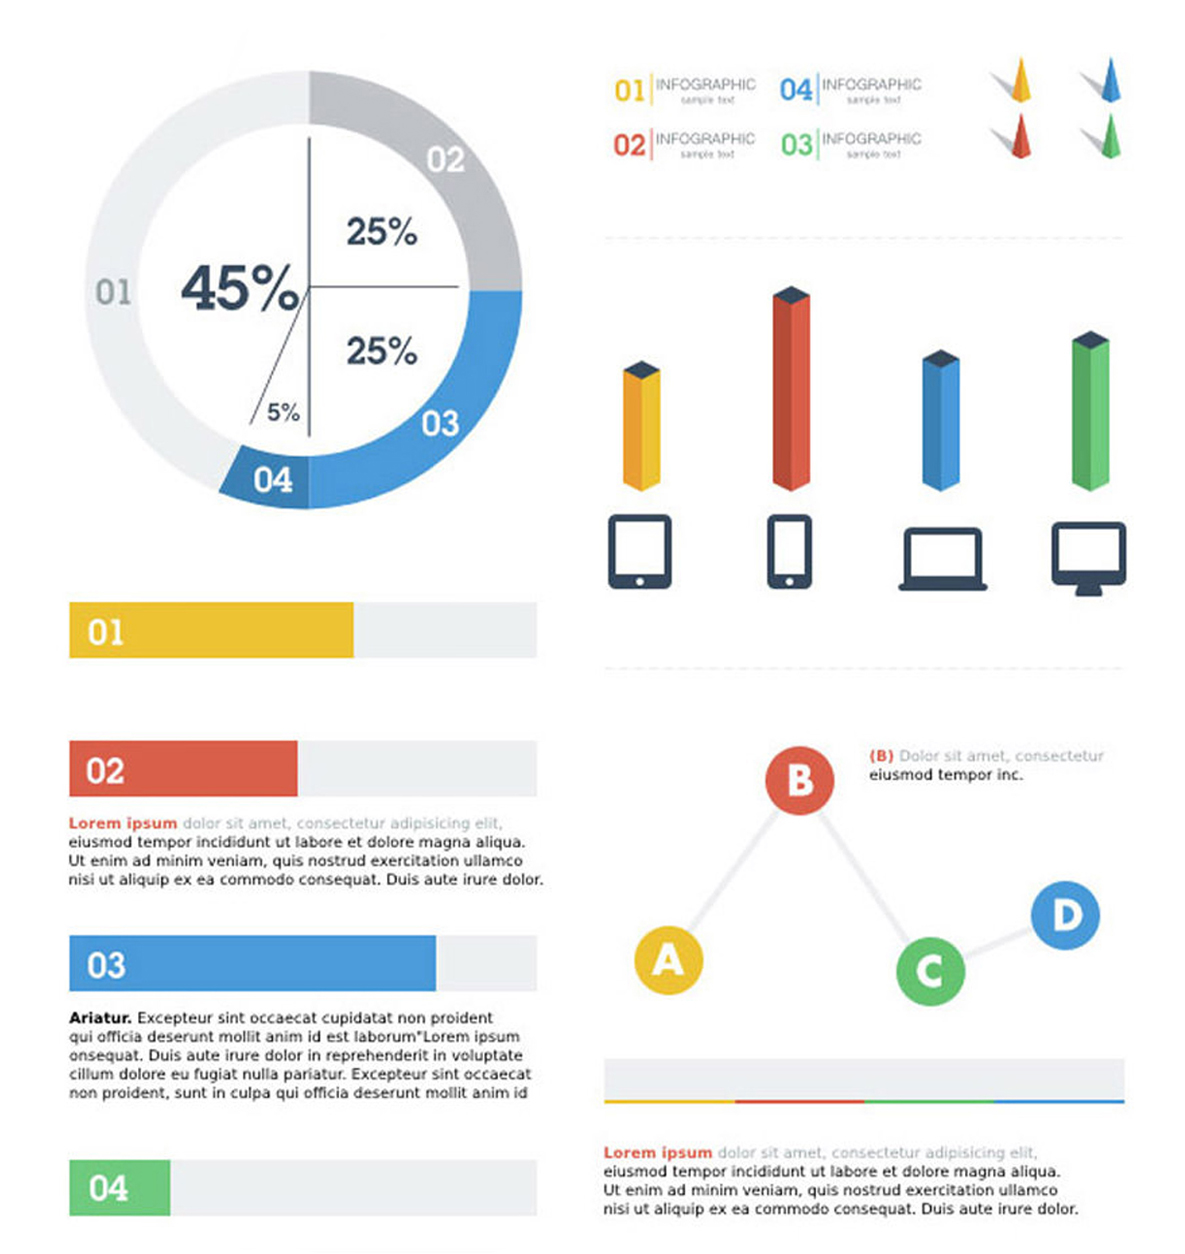
\includegraphics[height=10cm]{images/infographic.jpg}
    \caption{Exemple d'une infographie \footnotemark}
    \label{fig:2.3}
\end{figure}
\footnotetext{source : \url{https://www.hongkiat.com/blog/infographic-design-kit/}}
\subsubsection{1. Infographie d'information}
L'infographie informationnelle se distingue par son utilisation de texte supérieure à la moyenne par rapport à d'autres types d'infographie. Le graphique peut être amélioré par des icônes, des formes, des couleurs et d'autres éléments visuels, mais dans l'ensemble, l'accent est mis sur les mots.

\subsubsection{2. Infographie de la chronologie }
L'infographie de la chronologie décrit les événements ou les actions dans un ordre chronologique. Ils sont souvent utilisés pour démontrer le développement d’un produit, une tendance historique ou l’évolution d’une idée. L'infographie de la chronologie utilise des icônes, des images et des éléments graphiques pour transmettre le message. Le format de la timeline peut être vertical, horizontal ou sinueux. Les infographies verticales et chronologiques sinueuses sont généralement plus faciles à lire. Une infographie de chronologie horizontale convient mieux aux affiches, aux présentations et aux environnements où l'espace n'est pas une contrainte.

\subsubsection{3. Infographie de graphiques }
L’infographie de graphiques a un graphique comme pièce maîtresse de la visualisation des informations. Des couleurs, des formes et des icônes peuvent être ajoutés à des fins d'emphase et/ou d'explication. Les graphiques fonctionnent mieux lorsqu’il est effectué une comparaison élémentaire d'éléments. 

\subsubsection{4. Infographie de graphiques en secteurs}
Les graphiques en secteur apparaissent assez souvent dans l'infographie, car ils sont très utiles quand il faut montrer des pourcentages d'un tout. Il est préférable d'utiliser les graphiques en secteur pour afficher des différences au sein d'un groupe en fonction d'une variable. Dans l'infographie, les graphiques en secteur viennent dans beaucoup de variantes et de styles pour montrer les différents composants d’un élément ou pour comparer une valeur à plusieurs autres valeurs.

\subsubsection{5. Infographie de processus }
L’infographie de processus décrit les processus de prise de décision. Les infographies de processus sont également appelées arbres de décision ou organigrammes. Chaque étape est liée à la suivante par des lignes et des flèches directionnelles. 

Alors qu'il existe différents types d'infographies, certains éléments sont essentiels pour rendre une représentation visuelle des données qualifiée d'infographie. Pratiquement toutes les infographies utilisent chacune d’elles dans une certaine mesure (couleurs, polices, icônes et images).

\subsection{Géomatique et Cartographie}
Le terme géomatique est un néologisme composé de « géo » (pour géographie) et de « matique » (pour informatique). C’est la discipline ayant pour objet « la gestion des données à référence spatiale et qui fait appel aux sciences et aux technologies reliées à leur acquisition, leur stockage, leur traitement et leur diffusion» \cite{11}. En somme, la géomatique est le domaine de l’informatique auquel se rattache les SIG (Système d’Information Géographique). La cartographie incorpore trois dimensions sous-jacentes \cite{11}:

\begin{itemize}
\item \textbf{Une dimension informatique:}  aujourd’hui, sauf dans la volonté de produire une image originale à forte valeur artistique, plus personne ne réalise de carte à la main mais via des logiciels spécialisés. 
\item \textbf{Une dimension spatiale:}  l’information géographique (localisée dans l’espace) est la matière première du cartographe. 
\item \textbf{ Une dimension graphique:} cartographier, c’est dessiner l’espace géographique, ses continuités, ses ruptures. C’est mettre sur écran une représentation schématique de l’espace géographique.
\end{itemize} 
Le processus de conception cartographique concerne une transformation systématique des données spatiales en un affichage spatial multidimensionnel. Ce processus est généralement exécuté en appliquant des méthodes de «conception cartographique scientifique», ainsi que des règles esthétiques.

En cartographie, une carte peut fournir un aperçu général d’une zone géographique avec différents niveaux de détail; le niveau et la surface dépendent du point de vue et de la fonction du cartographe. Les cartographes utilisent plusieurs méthodes pour créer des cartes thématiques, mais quatre méthodes sont plus courantes:
\subsubsection{1. Les cartes à points (Dot Map)}
Les cartes à points sont un moyen de détecter les modèles spatiaux ou la distribution des données sur une région géographique, en plaçant des points de taille égale sur une région géographique.
Il existe deux types de cartes à points : un en un (un point représente un seul compte ou un objet) et un en plusieurs (un point représente une unité particulière, par exemple 1 point = 10 arbres).
Les cartes à points sont idéales pour voir comment les choses sont réparties sur une région géographique et peuvent révéler des motifs lorsque les points se regroupent sur la carte. Les cartes à points sont faciles à comprendre et donnent un meilleur aperçu des données, mais ne sont pas très utiles pour récupérer des valeurs exactes.
\begin{figure}[!ht]
    \centering
    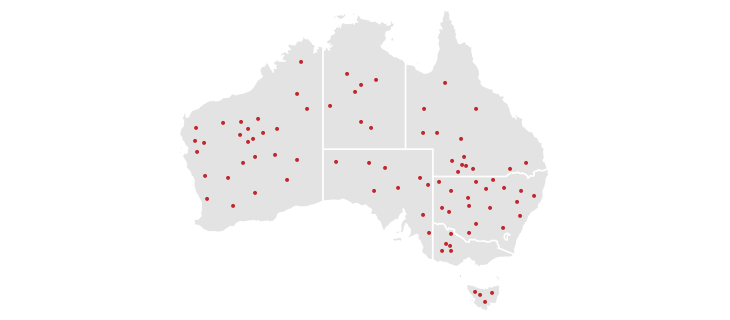
\includegraphics[height=5cm]{images/dot_map.png}
    \caption{Carte à point \footnotemark}
    \label{fig:2.4}
\end{figure}
\footnotetext{source : \url{https://datavizcatalogue.com/methods/dot_map.html}}
\subsubsection{2. Les cartes à bulle (Bubble Map)}
Avec cette carte de données, les cercles sont affichés sur une région géographique désignée, la surface du cercle étant proportionnelle à sa valeur dans le jeu de données. Les cartes à bulles permettent de comparer des proportions sur des régions géographiques sans les problèmes causés par la taille de la région, comme le montre la carte de Choropleth. Cependant, l'un des principaux défauts de la carte à bulle est que des bulles trop volumineuses peuvent chevaucher d'autres bulles et régions sur la carte. Il faut donc en tenir compte.
\begin{figure}[!ht]
    \centering
    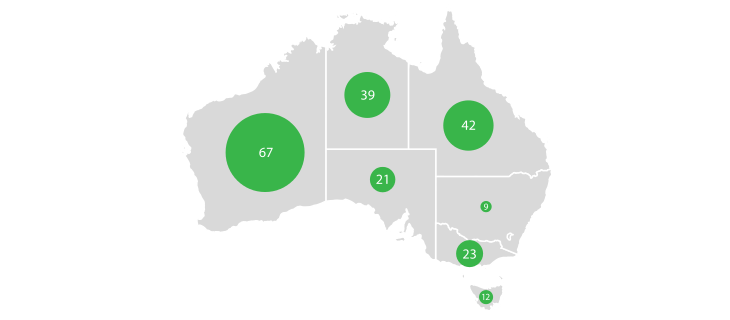
\includegraphics[height=5cm]{images/bubble_map.png}
    \scriptsize{source :\url{https://datavizcatalogue.com/methods/bubble_map.html}}
    \caption{Carte à bulle \footnotemark}
    \label{fig:2.5}
\end{figure}
\footnotetext{source : \url{https://datavizcatalogue.com/methods/dot_map.html}}
\subsubsection{3. Les cartes Choroplèthes (Choropleth Map)}
Les cartes Choroplèthes affichent des zones géographiques ou des régions divisées colorées, ombrées ou structurées par rapport à une variable de données. Cela fournit un moyen de visualiser les valeurs sur une zone géographique, ce qui peut montrer des variations ou des modèles sur l'emplacement affiché.
La variable de données utilise la progression de la couleur pour se représenter dans chaque région de la carte. En règle générale, il peut s'agir d'un mélange d'une couleur à une autre, d'une progression de teinte unique, transparente à opaque, claire à sombre ou d'un spectre de couleurs complet.
\begin{figure}[!ht]
    \centering
    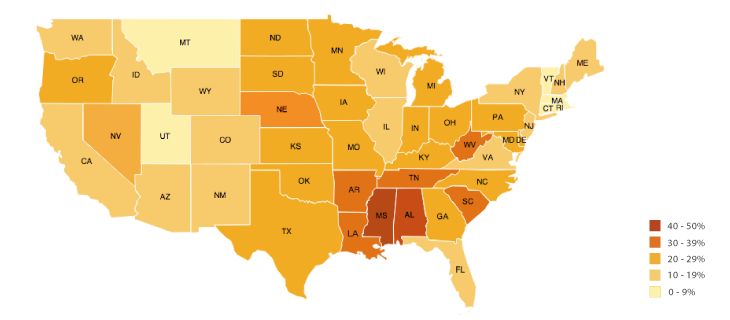
\includegraphics[height=5cm]{images/choropleth.png}
    \caption{Carte Choroplèthes \footnotemark}
    \label{fig:2.6}
\end{figure}
\footnotetext{source : \url{https://datavizcatalogue.com/methods/choropleth.html}}
\begin{figure}[!htb]
\begin{minipage}{0.46\linewidth}

\subsubsection{4. Les cartes thermiques (Heatmap)}
La figure~\ref{fig:2.7} montre les précipitations annuelles moyennes en Inde, en utilisant différentes nuances de bleu. Plus la nuance de bleu est sombre, plus les précipitations sont élevées.

Les cartes thermiques permettent de visualiser les données à travers des variations de coloration. Lorsqu'elles sont appliquées à un format tabulaire, les cartes thermiques sont utiles pour effectuer un examen croisé des données multivariées, en plaçant des variables dans les lignes et les colonnes, et en colorant les cellules du tableau.
Les cartes thermiques sont utiles pour afficher la variance entre plusieurs variables, révéler toutes les tendances, indiquer si des variables sont similaires les unes aux autres et pour détecter si des corrélations existent entre elles.
\end{minipage}\hfil
\begin{minipage}{0.35\linewidth}
\centering
    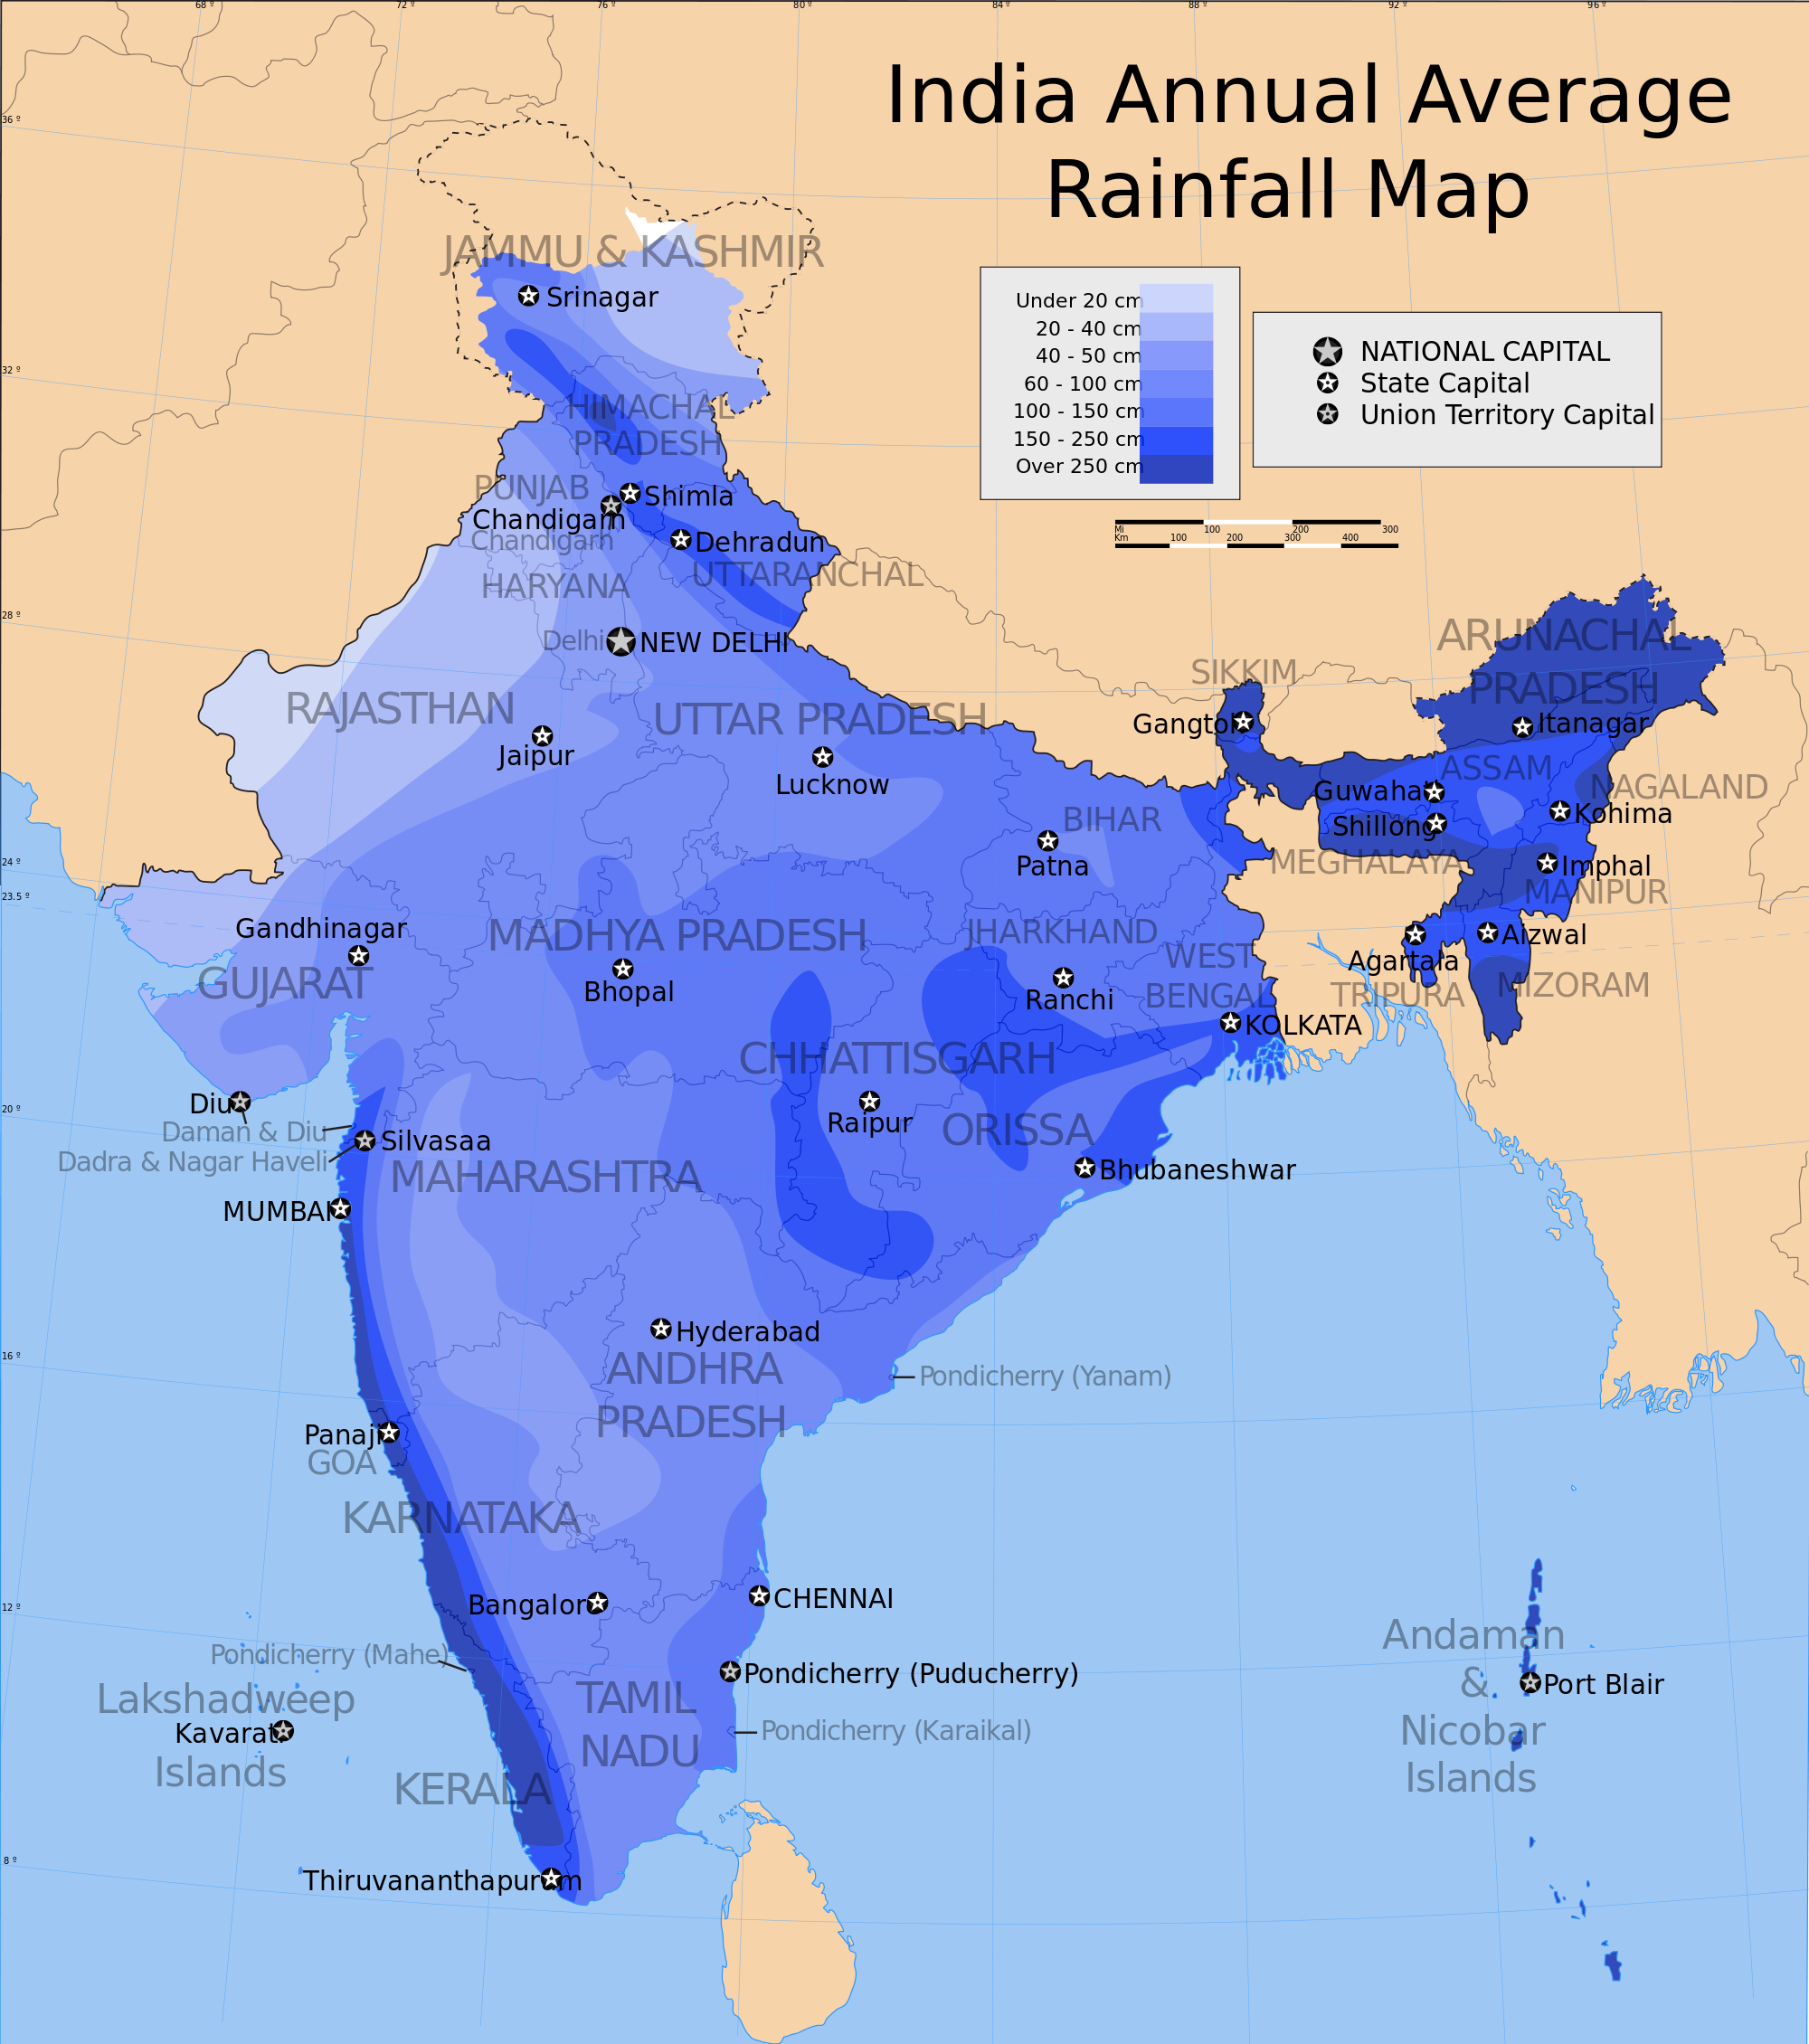
\includegraphics[height=8cm]{images/Heatmap.png}
    \caption{Carte thermique \footnotemark}
 \label{fig:2.7}
\end{minipage}
\end{figure}
\footnotetext{source : \url{https://blog.socialcops.com/academy/resources/7-techniques-to-visualize-geospatial-data/}}

En règle générale, toutes les lignes constituent une catégorie (étiquettes affichées à gauche ou à droite) et toutes les colonnes constituent une autre catégorie (étiquettes affichées en haut ou en bas). Les lignes et les colonnes individuelles sont divisées en sous-catégories, qui correspondent toutes les unes aux autres dans une matrice. Les cellules contenues dans le tableau contiennent des données catégoriques à code de couleurs ou des données numériques, basées sur une échelle de couleurs. Les données contenues dans une cellule sont basées sur la relation entre les deux variables de la ligne et de la colonne de connexion.

Une légende est nécessaire à côté d’une carte thermique pour que celle-ci puisse être lue avec succès. Les données catégorielles sont codées par couleur, tandis que les données numériques nécessitent une échelle de couleurs qui se mélange d'une couleur à l'autre afin de représenter la différence entre les valeurs hautes et basses. 
Les cartes thermiques peuvent également être utilisées pour afficher les modifications des données au fil du temps si l'une des lignes ou des colonnes est définie sur des intervalles de temps. Par exemple, utilisez une carte thermique pour comparer les changements de température au cours de l’année dans plusieurs villes, afin de déterminer les endroits les plus chauds ou les plus froids. Ainsi, les lignes pourraient répertorier les villes à comparer, les colonnes contiennent chaque mois et les cellules contiennent les valeurs de température.

\subsection{La Géovisualisation}
La géo-visualisation et l'analyse visuelle de données géospatiales sont devenues un centre d'intérêt pour la recherche, les industries, le gouvernement et d'autres organisations pour améliorer la mobilité, l'efficacité énergétique, la gestion des déchets et l'administration publique d'une ville intelligente \cite{12}.\\

La géovisualisation communique les informations géospatiales d'une manière qui, associée à la compréhension humaine, permet l'exploration des données et la prise de décisions. Les cartes statiques traditionnelles ont une capacité d'exploration limitée. La géovisualisation permet des cartes plus interactives, y compris la possibilité d'explorer différentes couches de la carte, d'effectuer un zoom avant ou arrière, de modifier l'aspect visuel de la carte et d’apporter des modifications à une carte en temps réel permettant aux utilisateurs d’ajuster les données cartographiées. La géovisualisation représente un ensemble de technologies et de pratiques cartographiques qui tirent parti de la capacité des technologies modernes. Il est important de rendre les données complexes plus claires et utiles grâce à une conception visuelle appropriée, par exemple en inventant de nouvelles métaphores visuelles, en créant des algorithmes d'analyse, etc. \\*
L'analyse visuelle intègre de nouveaux outils avec des techniques interactives innovantes et des représentations visuelles pour permettre une interaction homme-information. La conception des outils et des techniques repose sur des principes cognitifs et perceptuels. Cette science du raisonnement analytique fournit le cadre sur lequel il est possible de construire des technologies d'analyse visuelle stratégiques et tactiques pour l'analyse des menaces, la prévention et la réaction.
Les outils d'analyse visuelle doivent permettre différentes tâches d'analyse, telles que:

\begin{itemize}
\item Comprendre rapidement les situations, ainsi que les tendances et les événements qui ont généré les conditions actuelles.
\item Identifier les futurs possibles et leurs signes avant-coureurs
\item Surveiller les événements actuels pour détecter l'apparition de signes avant-coureurs et d'événements imprévus.\\
\end{itemize}

La gestion des données spatiales joue un rôle fondamental dans la conception de l’information urbaine. La conception de l'information urbaine est l'un des outils les plus importants dans l'analyse des processus urbains et dans la planification d'une ville intelligente.

Ces dernières années, différentes techniques de représentation des données spatiales ont été considérablement développées dans différents types de cartes (cartes de points, de lignes, de polygones, de cartes choroplèthes, de cartes isoplèthes, de cartogrammes, etc).\\ Les indicateurs spatiaux peuvent être représentés de différentes manières: en deux ou en trois dimensions, en fonction du caractère bidimensionnel ou tridimensionnel des phénomènes. Si le phénomène analysé a principalement deux dimensions, il est courant de le représenter en utilisant le même nombre de variables spatiales. 
La représentation consiste à faire des choix qui nécessitent un premier niveau d’analyse pour extraire la signification et la transmettre à l’utilisateur via une représentation graphique, telle que la carte ou la visualisation 3D illustré ci-dessous. 


\begin{figure}[!ht]
    \centering
    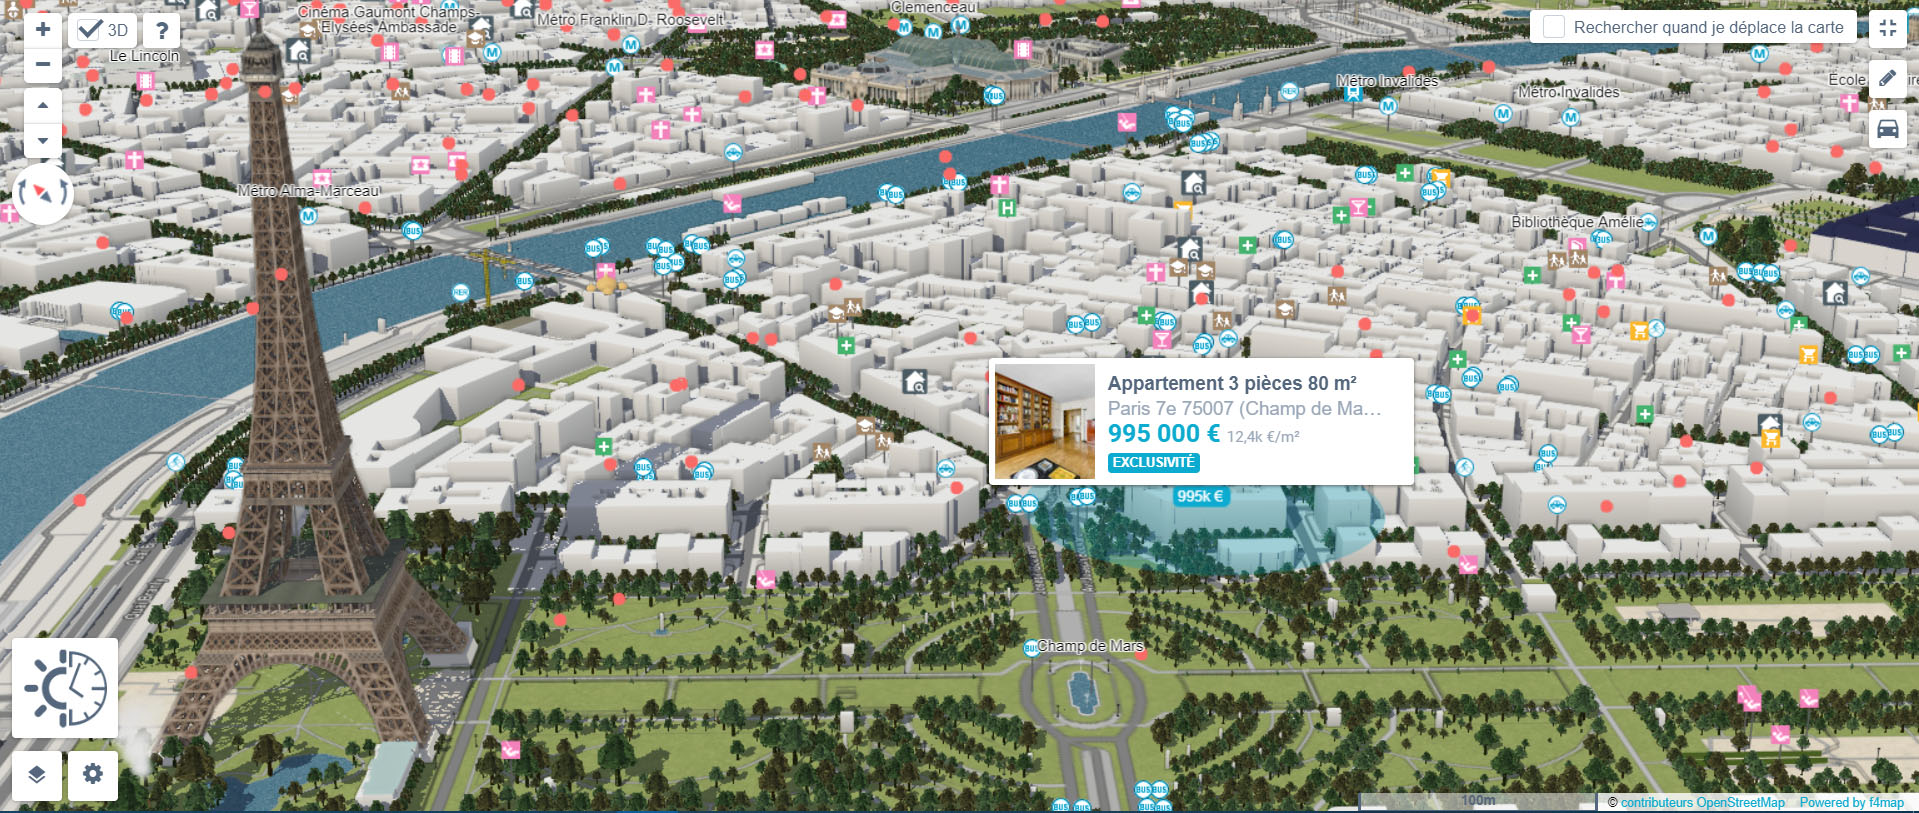
\includegraphics[height=6.6cm]{images/bienIci.jpg}
    %\scriptsize{source :\url{https:// }}
    \caption{capture d'écran du site Bien’Ici }
    \label{fig:2.9}
\end{figure}
La figure ~\ref{fig:2.9} présente une nouvelle approche pour la recherche immobilière, plus simple, plus rapide et plus agréable pour les internautes par l’entreprise Bien’Ici . Sa cartographie en 3D était développée par l’agence de jeux vidéos F4Map\footnote{ La carte F4 (F4Map) est une carte 3D basée sur Openstreetmap qui utilise la technologie WebGL } qui a modélisé la France entière en 3D. La carte passe automatiquement en 3D à partir d’un certain niveau de zoom. Toutes les annonces sont repérables sur la carte par un point rouge ou une étiquette de prix.  La carte en 3D permet de déplacer dans tous les sens afin de découvrir le logement et le quartier sous tous les angles.

%%%%%%%%%%%%%%%%%%%%%%%%%%%%%%%%%%%%%%%%%%%%%%%%%%%%%%%%%%%%%%%%%%%%%
\section{Outils de visualisation du Big Data: }
Les outils de visualisation de données sont exactement les armes dont nous avons besoin. Ces outils nous montrent diverses informations sur les données collectées. Les grands entreprises tels que Google et Microsoft collectent et manipulent des données volumineuses pour concevoir l'avenir de leurs stratégies commerciales. Cette section couvre certains outils de visualisation associés au Big Data. Les outils de visualisation sont diverses.  Plusieurs approches se sont dégagés selon le contexte. \\

\subsection{Approche de visualisation de JS}
\label{subsec:JS}
Cette approche contient l’ensemble des bibliothèques de Java Script spécialisées dans la visualisation de données. Elle aide les développeurs qui confectionnent des applications web ou mobile à visualiser les données dans leurs propres applications. 
Parmis les nombreuses bibliothèques Javascript, les six bibliothèques les plus utilisées sont décrites ci-dessous : 
\subsubsection{1. Data Driven Document «D3.js»}
D3.js est une bibliothèque Javascript permettant de visualiser le Big Data de la manière que le développeur souhaite. Une connaissance solide en Javascript du développeur est nécessaire pour donner une forme aux données collectées. 

D3.js est très complète avec beaucoup d’exemples à disposition, avec une personnalisation totale possible. Elle permet l’accès à des primitives SVG permettant toute innovation. Les données peuvent être sous différents formats, le plus souvent JSON,  CSV ou geoJSON. Ces principales caractéristiques sont : 

\begin{itemize}
    \item Prise en charge de nombreux types de graphiques, bien plus que la grande majorité des autres bibliothèques de graphiques JavaScript.
    \item Combine des composants de visualisation puissants et une approche de manipulation DOM basée sur les données.
    \item Facile à déboguer à l'aide de l'inspecteur d'éléments intégré au navigateur.
    \item Des centaines d'exemples.
    \item Glisser déposer , zommer et d'autre.
    \item D3 est une bibliothèque JavaScript open source pour les graphiques, qui est gratuite pour tout type d'utilisation.
    
\end{itemize}
\subsubsection{2. Chartist.js}
Chartist.js est une bibliothèque JS open source non intrusive qui peut également être utilisée pour créer des graphiques réactifs. Chartist convient aux utilisateurs qui ont besoin d’un graphique très simple (lignes, barres ou secteurs) et qui n’exigent pas beaucoup de visualisation de données. Les principales caractéristiques sont :
\begin{itemize}
\item \textbf{} Nombre de types de graphiques restreint
\item \textbf{} Possibilité d’ajouter des animations.
\item \textbf{} La documentation de l’API contient toutes les informations
\item \textbf{}  Nécessaires, mais peu pratique à utiliser et nécessitant de longs parchemins.
\item \textbf{} Permet d'utiliser des plugins pour étendre les fonctionnalités.
\item \textbf{} Utilise SVG pour dessiner les graphiques (compatibles à l’avenir).
Vieux navigateurs supportés.
\item \textbf{} Open source, gratuit pour tout type d’utilisation.
\end{itemize} 
\subsubsection{3. Chart.js}
Chart.js est une bibliothèque JavaScript simple et flexible pour la visualisation de données. C’est une excellente solution de base pour les développeurs qui ne nécessitent pas de nombreux types de graphiques et de fonctions de personnalisation, mais qui souhaitent que leurs graphiques soient nets, clairs et instructifs. Les principales caractéristiques sont : 
\begin{itemize}
\item \textbf{} Huit types de graphique: ligne, zone, barre, camembert, radar, polaire, bulle et diffusion.
\item \textbf{} Tous les types de graphique peuvent être personnalisés et animés.
\item \textbf{}  Lorsqu'ils sont utilisés en ligne, tous les graphiques sont réactifs.
\item \textbf{} La fonctionnalité peut être étendue grâce à l'utilisation de plugins.
\item \textbf{} Une documentation assez riche.
\item \textbf{} Support via Stack Overflow.
\item \textbf{} Les navigateurs supportent IE9 +.
\item \textbf{} Une bibliothèque de graphiques JS open-source gratuite. Publié sous licence MIT.
\end{itemize} 
\subsubsection{4. HighCharts}
Highcharts est l’une des bibliothèques de graphiques JavaScript les plus complètes et les plus populaires, basée sur HTML5, avec un rendu au format SVG / VML. Il est léger, prend en charge un large éventail de types de graphiques et garantit des performances élevées. Les principales caractéristiques sont : 
\begin{itemize}
\item \textbf{} Une utilisation du JavaScript pur. 
\item \textbf{} Les données peuvent être chargées en externe.
\item \textbf{} Une documentation robuste, une référence API et une présentation de la communauté.
\item \textbf{} Une exploration des données du graphique et d'autres options d'interactivité.
\item \textbf{} Une utilisation possible avec différentes framework front-end tels que React, Angular, Meteor, .NET, iOS, etc.
\item \textbf{} Une exportation au format PNG, JPG, PDF ou SVG.
\item \textbf{} Gratuit pour les organismes à but non lucratif. Payé pour un usage commercial (à partir de 50 \$).
\end{itemize} 

\subsubsection{5. C3.js}

C3.js est une autre bibliothèque de diagrammes réutilisable. C3.js est Open Source et est basé sur la bibliothèque D3.js qui est actuellement très complète et permet de réaliser une grande diversité de rapports. Les principales caractéristiques sont :
\begin{itemize}
\item \textbf{} Grand nombre d’outils de cartographie basés sur D3.
\item \textbf{} Les graphiques sont interactifs et peuvent être dynamiques (onclick, onmouseover, etc). 
\item \textbf{} Il est également possible de les imprimer en PDF.
\item \textbf{} Pouvoir activer ou désactiver le zoom sur un graphique, charger des données depuis une url ou un fichier de type CSV, inverser les abscisses et ordonnées, modifier la « tooltip ».
\item \textbf{} Il fournit un certain nombre d'API et de callbacks pour mettre à jour le graphique.
\item \textbf{} Une bibliothèque de graphiques JS open-source gratuite. Publié sous licence MIT.
\end{itemize} 

\subsubsection{6. Plotly.js}
Plotly.js est une bibliothèque JavaScript de haut niveau, gratuite et à code source ouvert. Il est basé sur D3.js et WebGL. Il peut donc être utilisé pour créer de nombreux types de graphiques, notamment des graphiques 3D aux graphiques statistiques. Les principales caractéristiques sont : 
\begin{itemize}
\item \textbf{} 20 types de graphiques pouvant être intégrés à des sites Web ou utilisés pour créer des présentations dynamiques.
\item \textbf{} Utilisée comme une bibliothèque de graphiques basée sur un navigateur pour Python, R et MATLAB, en résumant des graphiques en une structure JSON déclarative.
\item \textbf{} Permet d'utiliser des feuilles de calcul Excel ou de se connecter à votre base de données.
\item \textbf{} Exportation de graphiques en PNG et JPG; EPS, SVG et PDF sont disponibles sur abonnement.
\item \textbf{} Documentation complète sur les API.
\item \textbf{} Open-source, bibliothèque gratuite.
\end{itemize} 
\subsubsection{7. Nvd3}
NVD3 est une bibliothèque Javascript visant à créer des graphiques et des composants réutilisables pour D3.js, en offrant les mêmes fonctionnalités puissantes, mais beaucoup plus simple à utiliser. Elle permet de gérer des ensembles de données complexes et de créer des visualisations avancées.

\subsection{Approche de visualisation des BI}
Les outils d'aide à la décision ont pour objectif d’aider à comprendre les tendances et à tirer parti de données pour permettre de prendre des décisions commerciales stratégiques.
Ces outils permettent de réaliser des graphiques, des présentations et des tableaux de bord en toute simplicité. Les analyses de données peuvent être effectuées à l’aide de JavaScript, Python, R, Matlab, Jupyter ou encore Excel. 
Cependant, avec le nombre important d’outils de BI sur le marché, le démarrage du processus de sélection peut être difficile. Parmi ceux-ci , les trois BI les plus utilisés selon les statistiques sont \cite{14} : 
\subsubsection{1. Sisense}
Le logiciel de BI Sisense permet aux entreprises de rassembler, d’analyser et de visualiser des données pouvant être utilisées pour prendre de bonnes décisions et d’élaborer des plans stratégiques. L'outil regroupe toutes les informations nécessaires dans un tableau de bord unique avec sa fonctionnalité de glisser-déposer et fournit une vue granulaire des données. Les utilisateurs peuvent proposer une analyse fiable en utilisant des rapports visuels comme base, ce qui simplifie considérablement le processus. L’interface de la plate-forme est facile à utiliser, permettant aux utilisateurs d’apprendre rapidement et facilement la navigation dans les systèmes. Les principaux avantages sont :
\begin{itemize}
\item \textbf{Utilisation rationnelle des ressources:}  la technologie In-Chip de Sisense optimise les ressources déjà existantes sur une machine en déterminant la meilleure utilisation possible de sa capacité pour stocker, compresser et accéder à plus de données plus rapidement. Sisense est capable de déplacer des données 50 à 100 fois plus rapidement que les solutions en mémoire en utilisant la mémoire disponible dans la CPU.
\item \textbf{Performances:}  Sisense est conçu avec une base de données en colonnes évolutive et optimisée en mémoire, capable de gérer des téraoctets de données et des dizaines de requêtes simultanées. Cela permet aux non-techniciens de joindre facilement des données provenant de sources multiples et de créer des visualisations et des rapports interactifs.
\item \textbf{ Réponse plus rapide:} le produit utilise la technologie BI d'accélération pour scinder chaque requête en blocs de requête et chaque bloc de requête est mis en cache individuellement. Cela se traduit par une réponse plus rapide aux nouvelles requêtes et permet au cache de rester efficace même lorsque le nombre d'utilisateurs et de requêtes augmente.
Consolidation de graphiq
\item \textbf{Consolidation de graphiques provenant de sources multiples:}  le pouvoir unique de Sisense est qu’il reconnaît et rassemble automatiquement des graphiques et des tableaux de différentes sources de données, puis combine les données qu’ils contiennent sans les préparer.
\end{itemize} 
\subsubsection{2. Tableau}
 Tableau aide les entreprises à visualiser et à comprendre les données. Il permet aux organisations de connecter, visualiser et partager des données via un PC ou un iPad. Les utilisateurs peuvent facilement créer des tableaux de bord, les publier et même les partager avec leurs collègues, partenaires et clients sans avoir besoin de connaissances en programmation. \\
 Le logiciel peut se connecter à de nombreuses sources d’information et importer et visualiser des informations dans un délai très court. Le logiciel est intuitif, facilitant l’utilisation et permettant l’analyse de données à l’aide de la fonctionnalité glisser-déposer. Il favorise la collaboration en permettant l’analyse de groupe et en informant tous les membres de l’équipe à tout moment. Les utilisateurs peuvent également accomplir des tâches pratiquement n'importe où et à tout moment, grâce à l'application mobile native.  Les principaux avantages sont :
 \begin{itemize}
\item \textbf{Glisser-déposer :} Tableau a été l'un des premiers systèmes de BI à présenter des tableaux de bord analytiques intuitifs dans lesquels les utilisateurs peuvent manipuler des données avec un simple mécanisme de glisser-déposer.
\item \textbf{Interactions de tableau de bord à tableau de bord :}  avec Tableau, il est possible de copier différents éléments de tableau de bord et les transférer dans d'autres classeurs. 
\item \textbf{Authentication SAML\footnote{Security assertion markup language (SAML) est un standard informatique définissant un protocole pour échanger des informations liées à la sécurité. Basé sur le langage XML, SAML a été développé par OASIS.} :} il s’agit d’une méthode open source permettant de créer une expérience de connexion unique. Ceci permet à Tableau de se connecter à n’importe quelle application / système tierce.
\item \textbf{Création avec Web mobile:}  Tableau affichera non seulement les données sur les appareils mobiles, mais il permettra également de modifier les vues existantes, d'analyser les données et d'enregistrer les nouvelles versions avec une application dédiée.
\end{itemize} 
\subsubsection{3. Power BI}
Microsoft Azure Power BI est un logiciel développé et prise en charge par Microsoft pour les besoins en matière de veille stratégique et d'analyse. Au cœur de Power BI se trouve un service en ligne offrant diverses options d’interaction, ainsi que plusieurs accès permettant la connexion aux données fournies.
Les principaux avantages sont :
\begin{itemize}
\item \textbf{Personnalisation riche des tableaux de bord :}  MS Power BI offre une expérience utilisateur unifiée avec des tableaux de bord et des rapports personnalisés qui répondent aux besoins exacts de l'utilisateur. 
\item \textbf{Géo-cartes :} Les visualisations de géo-cartes interactives sont également renforcées par Bing Maps.
\item \textbf{Publication sécurisée de rapports:}  la configuration de l'actualisation des données est automatique et la publication des rapports est rapide, permettant ainsi à tous les utilisateurs de bénéficier des dernières informations.
\item \textbf{Pas de contraintes de mémoire et de vitesse:} Pas de contraintes de mémoire et de vitesse: la récupération et l’analyse des données est rapide, en éliminant les contraintes de mémoire et de vitesse.
\item \textbf{Aucune assistance technique spécialisée n’est requise:}  l’utilisateur peut tirer parti des avantages des enquêtes et les analyses agiles sont offertes par Power BI, en éliminant ainsi le besoin d’une assistance technique spécialisée.
\item \textbf{La fonction de questions / réponses (Q \& R):} il est constitue un avantage pour réaliser une BI en libre service.
\item \textbf{Innovation constante:}  le produit Power BI est mis à jour presque tous les mois avec de nouvelles fonctionnalités.\\
\end{itemize} 
Au total, il existe plus de 20 solutions BI sur le marché. Trois outils présentés ci-dessus font partis des solutions leaders. Il est très difficile aujourd’hui de faire un comparatif de tous ces produits. Cependant, ces solutions peuvent être classées sous deux catégories.
\begin{itemize}
\item \textbf{} Les solution BI intégrées, tels que Oracle Business Intelligence Foundation Suite, SAP BusinessObjects et IBM Cognos qui sont les leaders en matière d’ERP et qui intègrent leur couche BI dans leur produit pour la génération des rapports prédéfinis. Ces solutions sont plutôt adaptées aux grandes entreprises.
\item \textbf{} Les solutions d’exploration des données, tels que les produits dédiés à l’informatique décisionnelle et les outils offrant une fonction BI en self-service comme la suite SQL de microsoft, Qlik, Tableau, Tibco, Microstratégy, etc. 

\end{itemize} 

\subsection{Approche de visualisation de SIG}
La visualisation de données par la cartographie est devenue un moyen essentiel pour les villes intelligentes de tirer parti des données recueillies à partir de diverses technologies ou d’applications intelligentes. Les cartes de système d'information géographique (SIG) fournissent des éléments visuels faciles à assimiler et qui peuvent aider les villes à déterminer les zones nécessitant certains aménagements ou services, ainsi que les meilleurs plans de répartition des ressources.
Certains outils de cartographie sont destinées à des analyses de niche, d'autres à des analyses plus étendues, telles que les réparations nécessaires dans une ville. Bon nombre de ces applications vont au-delà du traçage des données existantes et fournissent également une analyse prédictive pour aider à prévenir et à résoudre les futurs problèmes des villes.
Les logiciels SIG englobent un large éventail d'applications impliquant une combinaison de cartes numériques et de données géoréférencées. Les logiciels SIG peuvent être classés en différentes catégories.
Il existe deux catégories principales :  

\begin{enumerate}
\item \textbf{Logiciel open source} 
\begin{itemize}
     \item SIG de bureau tels que GRASS GIS, MapWindow GIS et QGIS.
     \item Serveurs de cartes Web tels que GeoServer, MapServer et Mapnik.
     \item Systèmes de gestion de bases de données spatiales tels que PostGIS, SpatiaLite et TerraLib.
     \item Structures de développement de logiciels et bibliothèques (pour les applications Web) tels que GéoBase (logiciel Telogis GIS), Geomajas, OpenLayers et Leafletjs (Bibliothèque JavaScript ouverte pour des cartes interactives adaptées aux mobiles). 
   \end{itemize}
\item \textbf{Logiciel SIG commercial } 
\begin{itemize}
     \item SIG de bureau tels que les produits Esri qui comprennent les services ArcMap, ArcGIS, ArcSDE, ArcIMS, ArcWeb et ArcGIS Server.
     \item Systèmes de gestion de bases de données spatiales tels que PostGIS, MySQL, Microsoft SQL Server, Oracle Spatial et Informix. 
     \item SIG en tant que service :
     \begin{enumerate}
         \item \textbf {SaaS} : logiciel en tant que service tels que : ArcGIS Online CartoDB Mapbox (fournisseur de cartes en ligne personnalisées pour sites Web)
         \item \textbf {PaaS} : Plate-forme en tant que service tels que : API Google Maps Javascript version 3, API de flux de données et Microsoft Bing Geocode 
         \item \textbf {DaaS} : Données en tant que service tels que : Cartes Apple, Google Maps, OpenStreetMap et Microsoft Bing Maps 
       \end{enumerate}
   \end{itemize}
\end{enumerate} 
Parmi ces logiciels de bureau, ArcGIS et QGIS sont les plus connus. 

\subsubsection{1. ArcGIS}
ArcGIS est une puissante plate-forme de cartographie et d'analyse conçue pour aider les entreprises à explorer des informations et à partager des informations localisées. Le logiciel utilise des outils contextuels de raisonnement spatial et de cartographie pour les industries, les éducateurs, les développeurs et les gouvernements du monde entier.
Ce programme bien conçu comporte des fonctionnalités haut de gamme utilisant le système d’information géographique (SIG) pour résoudre des problèmes. L'ensemble unique de capacités comprend: l’analyse spatiale, la cartographie et la visualisation, le SIG 3D, l’imagerie et la télédétection, le SIG en temps réel, et la collecte et gestion de données. Les fonctionnalités appliquent l'analyse des lieux aux pratiques commerciales pour créer une compréhension plus profonde et aider à visualiser rapidement la manière dont les informations commerciales sont connectées. ArcGIS libère tout le potentiel des données dans chaque organisation pour révéler des informations plus profondes. Il fournit un ensemble unique d'outils contextuels qui aident les organisations à visualiser et à analyser des données. En outre, il aide les organisations à partager leurs points de vue et à collaborer via des cartes, des applications et des rapports.
ArcGIS utilise du système d’information géographique (SIG) qui aide les organisations de toutes tailles à interroger, analyser, visualiser et interpréter les données afin de mieux comprendre les relations, les tendances et les modèles. Le système offre une meilleure communication, une meilleure tenue des dossiers, des économies de coûts et une meilleure prise de décision.
ArcGIS a de nombreux excellentes fonctionnalités tel que la fonctionnalité d'analyse qui constitue le pivot de la plate-forme ArcGIS. Cette fonctionnalité aide à identifier un emplacement commercial idéal, à planifier de meilleures communautés et à réagir plus rapidement dans toutes les situations critiques.

\subsubsection{2. QGIS}

Quantum GIS (QGIS) est un système d’information géographique open source, multi-plateforme et convivial conçu pour la visualisation, la modification et l’analyse de données géospatiales. Cette plate-forme est libre d'utilisation et peut gérer plusieurs fonctionnalités et formats de bases de données. Ses plugins principaux fournissent un nombre croissant de capacités.
Cette outil de SIG permet de visualiser des données, des données de superposition vectorielles \footnote{Les données vectorielles sont constituées de points individuels qui sont stockés sous forme de paires de coordonnées (x, y) pour les données 2D.} et raster \footnote{Les données raster sont constituées de pixels (ou de cellules) et chaque pixel est associé à une valeur.} dans divers formats. Cela permet également de créer, éditer, gérer et exporter des couches de données, vectorielles et raster dans de nombreux formats. Son interface utilisateur conviviale simplifie l'exploration des données et la composition des cartes. L'analyse de données spatiales est disponible dans des bases de données spatiales. En attendant, son architecture de plug-in extensible et ses bibliothèques peuvent être utilisées pour exploiter le logiciel en fonction de nos besoins.
En outre, le logiciel fonctionne sur de nombreux systèmes d'exploitation, notamment: Mac, Windows, Unix, Linux et Android. Cette plate-forme n'est pas seulement un SIG de bureau, elle fournit également une application serveur, un navigateur de fichiers spatiaux et des applications Web.


Il permet d'explorer de manière interactive les données spatiales et de composer des cartes à l'aide de l'interface graphique conviviale. L'interface utilise de nombreux outils, notamment le gestionnaire de base de données, les signets spatiaux, le navigateur QGIS, les outils d'annotation, le panneau de présentation, le composeur de carte, la reprojection à la volée, etc.

QGIS facilite également l'analyse des données spatiales sur toutes les bases de données et autres formats pris en charge par OGR. Le logiciel propose des outils d'échantillonnage, d'analyse vectorielle, de géotraitement, de gestion de base de données et de géométrie. Un autre avantage est la possibilité d'étendre les fonctionnalités de QGIS à l'aide de plugins. Les bibliothèques de plugins extensibles et l'architecture facilitent l'adaptation de la plate-forme aux besoins spécifiques. En outre, il est plus facile de créer des applications supplémentaires en utilisant Python ou C ++.

\section{Etude comparative sur les approches }
\label{sec:comparative}
Il existe de nombreux outils de visualisation du Big Data, qui sont classé selon le contexte en trois catégories. Au sein de ces catégories, les outils de visualisation de données sont également classé en fonction de leur spécialité. 
Premièrement, les puissants outils de BI, tels que Tableau, permettent de visualiser, récupérer, analyser et documenter des données. Les outils de BI sont conçus pour rendre le flux de données gérable, permettant ainsi aux organisations, grandes ou petites, de transformer des données non structurées en actions exploitables sans besoin des experts de base de données ou des développeurs.
Deuxièmement, les bibliothèques de graphiques Javascript tels que D3js sont des outils de développement, principalement des bibliothèques des APIs ou des modules de langage de programmation. Ces outils sont utilisés pour étendre une application à l’aide de méthodes fournies ad hoc par la bibliothèque. 
Troisièmement, les outils de SIG tels que ArcGIS sont à l’origine de nombreux services de géolocalisation basés sur l’analyse des données et leur visualisation. Pour le développement urbain et sa durabilité, la technologie SIG a la capacité d’être utilisée pour piloter des systèmes d’aide à la planification, à l’aménagement du territoire, la gestion des infrastructures et réseaux, le transport,la logistique, l’assurance, les télécommunications, l’ingénierie, l’éducation et la recherche, etc. 

Après avoir décrit les principales approches caractérisant les outils de visualisation, il est nécessaire de dégager des critères pour comparer ces différents outils. Voici une description de ces critères de comparaison 
\begin{enumerate}
  \item \textbf {Catégorie de logiciel }: Il représente la typologie de la solution analysée. Il distingue une application de bureau (application autonome sans mécanisme d'extension), une application ou des services Web, une bibliothèque de logiciels (par exemple, une bibliothèque Javascript pour le Web), un framework logiciel (une application logicielle complexe avec un plugin ou mécanisme basé sur des add-ons pour l'étendre, afin de connecter le framework à une solution existante pour le stockage de données ou l'analyse). 
  \item \textbf {Technique de visualisation } : Il répond à la question ( Pour quel type d’objet graphique l’outil est-il conçu?). Ainsi, il renseigne sur l'objet graphique principal ou le widget pris en charge par l'outil. De nombreuses solutions ne se limitent pas à un seul objet graphique, mais généralement, il existe un ou plusieurs widgets pris en charge par l’outil. Par exemple, Plotly est conçu pour les widgets de graphique, alors que Polymaps pour les cartes.
  \item \textbf {Système d'exploitation} : Le système d'exploitation (par exemple, Linux, Windows, Mac OS X) sur lequel l'outil est exécuté.
  \item \textbf {Licence} : Ceci informe sur la licence de la solution, commerciale et open source sous diverses licences (Licence Apache, GNU GPL,MIT etc.).
  \item \textbf {Évolutivité } : Ce critère concerne les mécanismes de l’évolutivité horizontale des outils afin de prendre en charge de très grands ensembles de données. Certaines solutions concernent, par exemple, la possibilité de connecter le logiciel à 
  \item \textbf {Extensibilité} : Ce critère concerne les mécanismes d'extension de l'outil via des add-ons ou des plugins, ainsi que la possibilité de le connecter à une solution de stockage existante. Par exemple, Plotly peut être connecté à Matlab ou à R, à l’aide de connecteurs clients spécifiques. 
  \item \textbf {Dernière version et date de publication} : Pour déterminer si la solution est à jour ou non. Si la dernière date de publication n'est pas récente, il est possible que le produit ne soit plus pris en charge.
\end{enumerate}

Dans le cadre d’une ville intelligente, les trois approches peuvent être utilisées. Selon le contexte et le secteur de l’organisation, il sera privilégié une d’entre elles. 

Par exemple, si l’organisation est une entreprise qui est en train de développer une solution pour une smart city, il est indispensable de choisir un outil de développement tel que les bibliothèques de visualisation Javascript. Mais dans le cas d’une organisation qui souhaite gérer et visualiser une grande quantité de données avec des graphiques et des diagrammes, il est indispensable d’utiliser des logiciels de Business Intelligence tel que Tableau. 

Dans une ville intelligente, un nouveau développement urbain durable exige une visualisation urbaine complète et des modèles de ville en 3D offrant une visualisation urbaine étendue avec de nouvelles techniques d'interrogation de données. Le système d’information centralisé basé sur un système d’information géographique (SIG) fait le lien entre différents secteurs. Il constitue une plateforme intersectorielle intégrée pour collecter, gérer, compiler, analyser et visualiser des informations temporelles et géospatiales en vue d’une planification, d’un développement et d’une gestion urbains durables dans une ville intelligente. Il peut mieux expliquer l'interaction et la variation dans le temps des indicateurs de développement durable. 

Pour le développement durable des villes intelligente, le SIG possède des
caractéristiques intéressantes tels que : 
\begin{itemize}
  \item Sélection de site et acquisition de terres
  \item Planification, conception et visualisation
  \item Construction et gestion de projet
  \item Ventes et Marketing
  \item Facilité de gestion
  \item Opérations et rapports
\end{itemize}

Les SIG peuvent être utilisés tout au long du cycle de vie d'une ville intelligente: sélection du site, conception et construction, utilisation et maintenance. Le SIG est une technologie idéale qui peut évoluer dans tous les domaines, de l'actif individuel d'un bâtiment à un contexte pratiquement mondial reliant tous les aspects de la planification et du développement d'une ville intelligente.








%%%%%%%%%%%%%%%%%%%%%%%%%%%%%%%%%%%%%%%%%%%%%%%%%%%%%%%%%%%%%%%%%
\chapter{Cas pratique: visualisation du Big Data chez Datategy}
\section{Presentation de Datategy}
Datategy est une entreprise de 20 personnes. Il est spécialisé dans la science des données appliquée à la stratégie d'entreprise. La société est située à La Grande Arche, 1 parvis de la défense 92800, Paris, France.
Elle a été fondé par des scientifiques de données et des stratèges commerciaux en 2016.
La vision de Datategy consiste à extraire des informations pertinentes des données et à les transformer en une source majeure de prise de décision. Son objectif est d'amener les entreprises dans des organisations plus intelligentes et plus avisées et de tirer un avantage concurrentiel de l'utilisation efficace de leurs données.
Datategy est une entreprise qui propose deux services principaux: un service de conseil et un produit de ville intelligente pour le transport et le stationnement, appelé OctoCity.
Il couvre de nombreux secteurs: finance, énergie, services aux entreprises et produits de consommation. Afin de comprendre les spécificités des différents secteurs et d’optimiser efficacement l’utilisation de son expertise, la société s’intéresse à ces quatre secteurs.

\section{Presentation d’OctoCity solution}
La fraude coûte cher aux entreprises de services de transport. En France, le marché des transports coûte environ 800 millions d'euros et celui du stationnement environ 500 millions d'euros en 2017. La fraude représente environ 8 à 25\% du chiffre d’affaires des entreprises en France. Il augmente également chaque année d'environ 5\% .
Devant l’inefficacité des moyens existants Datategy a ainsi mis au point Octocity Transport, une solution innovante, basée sur un algorithme prédictif, d’intelligence Artificielle, une solution 100\% Cloud permettant de générer des itinéraires optimaux pour les agents. Il traite les réplications de données avec la technologie Cassandra pour une disponibilité à 100\%. Il est composé d'une application de site Web et d'une application mobile connectée en temps réel.
OctoCity est conçu pour les gestionnaires en permettant un suivi global des agents de contrôle sur le terrain et une analyse statistique de l'efficacité des tournées et des interventions à l'aide de l'application de site Web. Il est également conçu pour les agents de contrôle sur le terrain en permettant à l’application mobile de prendre des contraventions de stationnement et de consulter l’historique des contraventions de stationnement. Il oriente également les agents de contrôle vers les lieux où la fraude en matière de transport est plus importante en temps réel.


\section{Etude comparative entre les différent bibliothèque de la visualisation}
Dans le cadre de mon alternance, l’entreprise Datategy doit choisir une bibliothèque de visualisation qui répond à leurs besoins d’intégrer un dashboard avec différents graphiques et statistiques au sein du projet Transports. Un des objectifs de ce projet est de visualiser le nombre de contravention en fonction de différents critères tels que les stations, les lignes de bus, les arrondissements, etc. 
Initialement, l’entreprise fait le choix d’utiliser la bibliothèque D3js dont les avantages sont listés ci-dessous :
\begin{itemize}
  \item Gratuité et Open Source
  \item Flexibilité
  \item Dynamisme
  \item Gestion de données volumineuses
  \item Rédaction de code personnalisé
  \item Plugins
\end{itemize}

En réalisant des graphiques avec D3js, le codage prend beaucoup de temps et s’avère laborieux. Le code devient long et difficile à gérer.  D3js a notamment une longue courbe d'apprentissage. Cela demande aux développeurs beaucoup de temps pour apprendre les syntaxes. 
Concernant le chargement de l’application Web, D3js importera plus de 70 Ko de code pour les graphiques les plus simples. 
Ces points négatifs sont acceptable si l'objectif est de créer de nouvelles visualisations complexes. Cependant pour OctoCity, ce n'est pas le cas car il n’est pas nécessaire d’avoir beaucoup de types de graphiques différents et complexes. Pour faire des graphiques simples comme des donuts, des graphiques à barres, des graphiques linéaires, des diagrammes de dispersion, il est possible de les implémenter en utilisant une autre bibliothèque. 

Il existe de nombreuses bibliothèques de visualisation, tels que Nvd3, Chart.js, Chartist, Plotly, C3js, HighChart et vectory [voir section ~\ref{subsec:JS}]. Le choix s’est porté parmis ces 6 bibliothèques. Pour choisir, il est indispensable de dégager des critères de comparaison comme indiqué dans la section ~\ref{sec:comparative}.
Il existe de nombreux éléments comparables entre ces bibliothèques tels que :

\begin{enumerate}
  \item \textbf{La licence utilisée} : à l'exception des Highcharts, toutes ces bibliothèques sont sous licence MIT ou Apache. Cela signifie qu'elles peuvent être utilisées gratuitement. Il est également possible d’utiliser Highcharts gratuitement à des fins non commerciales. Sinon, il faut  acheter une licence.
  \item \textbf{L'enrichissement et la maintenance de la bibliothèque dans le temps} : ceci peut être évalué à travers la popularité et l’activité du dépôt Github des bibliothèques. Il existe plusieurs outils permettant d'évaluer la bibliothèque tel que npm trends. La figure ci-dessus montre le nombre d'étoiles, de forks  et d’issues pour chaque bibliothèque, ainsi que la dernière mise à jour. 
  \begin{figure}[!ht]
    \centering
    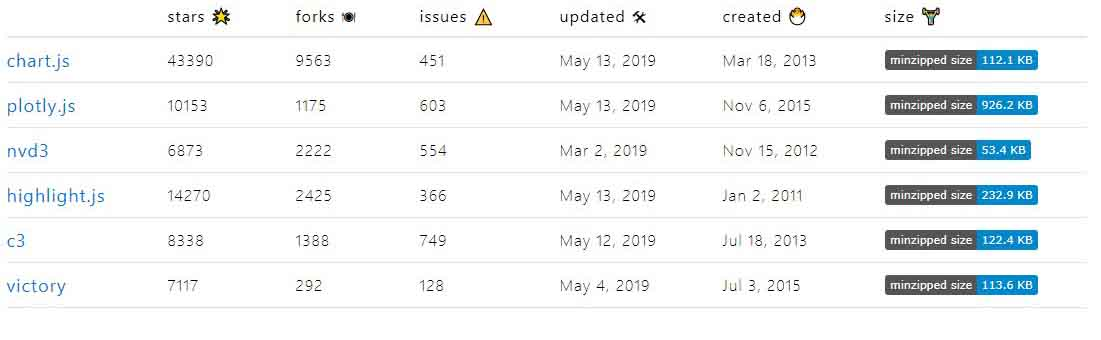
\includegraphics[height=4cm]{images/npm-trends-stat.jpg}
    \caption{Tableau comparatif des bibliothèque}
    \label{fig:3.1}
\end{figure}
  \item \textbf{Les techniques de visualisation} : Il en existe plusieurs tels que les graphiques 2D et 3D, les cartographies et les statistiques, etc. Toutes ces bibliothèques fournit des graphiques 2D tels que les donuts, les graphiques à barres, les graphiques linéaires, les diagrammes de dispersion, etc. De plus, la bibliothèque Plotly fournit aussi quelques graphiques en 3D et quelques types de cartographies tels que les cartes Choroplèthes, Nuages de points sur cartes et Cartes à bulles.
  \item \textbf{Les options de personnalisation} : tels que (titres, légendes, zoom, info-bulle, réactivité). Comparer les options de conception et de personnalisation est délicat. Chaque bibliothèque fournit des options personnalisées et il est difficile de les comparer. La table ci-dessus montre la présence des options pour chaque bibliothèque :
  \begin{figure}[!ht]
    \centering
    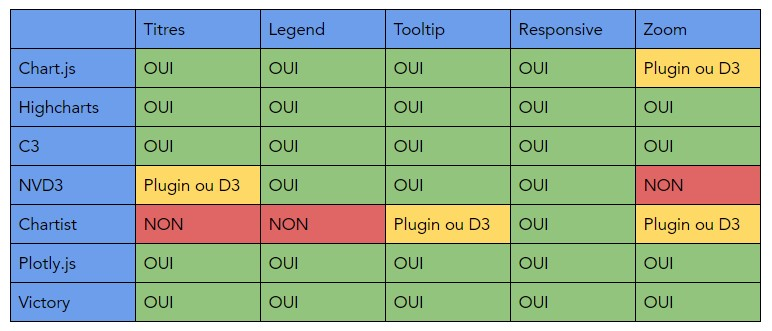
\includegraphics[height=5cm]{images/options-table.jpg}
    \caption{Tableau comparatif des bibliothèque selon les options personnalisation}
    \label{fig:3.2}
\end{figure}
  \item \textbf{Le nombre de téléchargements} : Consulter les téléchargements hebdomadaires sur NPM et les étoiles sur Github permet de savoir quelle est sa popularité.  La figure ci-dessus montre le nombre de téléchargement selon NPM trends. 
   \begin{figure}[!ht]
    \centering
    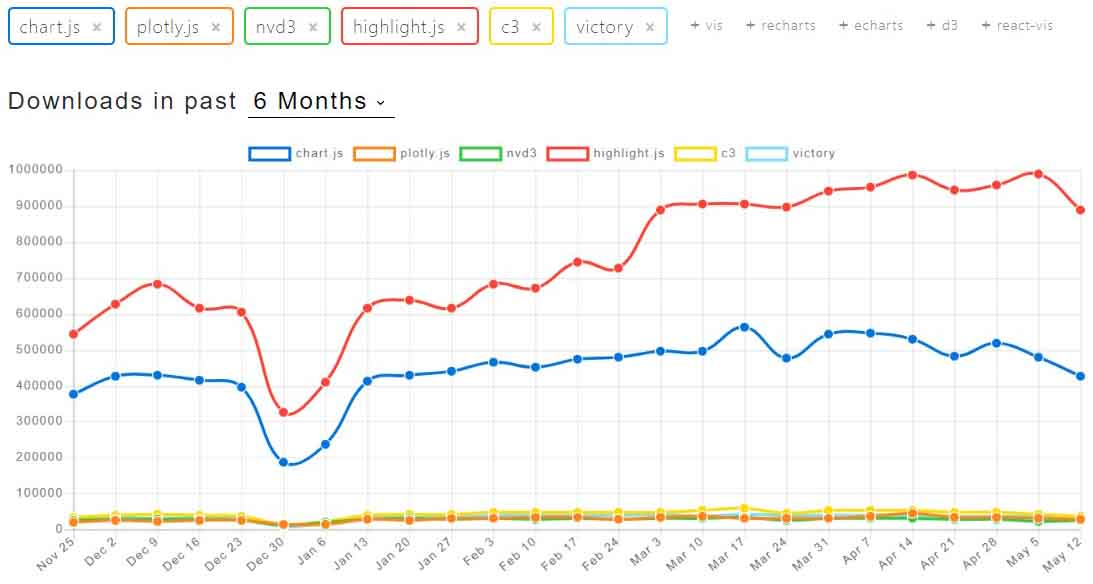
\includegraphics[height=6cm]{images/npm-trends-chart.jpg}
    \caption{Graphique comparatif des bibliothèque selon le nombre de téléchargement }
    \label{fig:3.3}
\end{figure}
  \item \textbf{ La maintenance active} : Elle est le meilleur moyen qui permet à la bibliothèque de passer d’une version nouvelle et expérimentale à une version stable et mature. Cela comprends des corrections des bugs réguliers et des améliorations supplémentaires. Pour cela, il faut consulter l'historique des commits et le Code Frequency (sous l'onglet Insights) sur Github, ainsi que vérifier la date de «dernière publication» sur le NPM. La table ci-dessous montre le nombre et la dernière date de commits par bibliothèque:
  \begin{figure}[!ht]
    \centering
    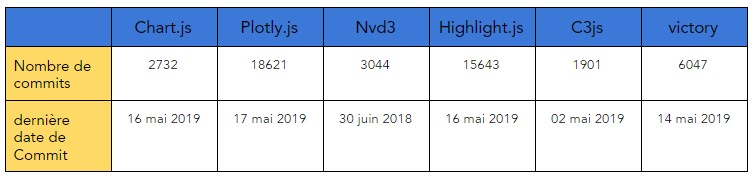
\includegraphics[height=3.3cm]{images/commit-table.jpg}
    \caption{Tableau comparatif des bibliothèque selon le nombre et la dernier date de Commits }
    \label{fig:3.4}
\end{figure}
  \item \textbf{Taille} : Il faut vérifier la taille du package en utilisant des outils tels que Bundlephobia qui indique la taille d'un package NPM, la durée de téléchargement estimée sur des réseaux lents, l'évolution de la taille de l'ensemble au fil des versions et la composition des dépendances.
  \item \textbf{Test de coverage} : Il est nécessaire de vérifier les badges de couverture sur NPM / Github et d’ouvrir les fichiers de test.
\end{enumerate}





\chapter{Bilan et conclusion}
\section{Bilan professionnel et personnel}
\section{Conclusion}


% \nocite{*}
% \bibliographystyle{plain}
% \bibliography{biblio} 
% \phantomsection 
\addcontentsline{toc}{chapter}{Bibliographie} 
\begin{thebibliography}{9}
\bibitem{0}
United Nations. \href{https://www.un.org/en/development/desa/population/publications/pdf/urbanization/the_worlds_cities_in_2016_data_booklet.pdf}{\emph{P.D.: The World’s Cities in 2016. United Nations}. [2016].} 

\bibitem{1} Paolo Neirotti, Alberto De Marco, Anna Corinna Cagliano, Giulio Mangano⇑, Francesco Scorrano \href{https://www.researchgate.net/publication/260015335_Current_trends_in_Smart_City_initiatives_Some_stylised_facts}{\emph{, Current trends in Smart City initiatives: some stylised facts. Cities}. [2013]} 

\bibitem{2}  Sandra Breux et Jérémy Diaz, \href{http://espace.inrs.ca/4917/1/Rapport-LaVilleIntelligente.pdf}{\emph{LA VILLE INTELLIGENTE Origine, définitions, forces et limites d’une expression polysémique}} [2017]

\bibitem{3} Taewoo Nam \& Theresa A. Pardo \href{https://inta-aivn.org/images/cc/Urbanism/background\%20documents/dgo_2011_smartcity.pdf}{\emph{, T.A.: Conceptualizing Smart City with Dimensions of Technology, People, and Institutions }.[2011]} 


\bibitem{4}IESE:\href{https://www.forbes.com/sites/iese/2019/05/21/these-are-the-smartest-cities-in-the-world-for-2019/}{\emph{Ranking The World’s ‘Smartest’ Cities. Forbes. Forbes.}} [2016]

\bibitem{5}Eiman Al Nuaimi, Hind Al Neyadi, Nader Mohamed and Jameela Al-Jaroodi \href{https://jisajournal.springeropen.com/articles/10.1186/s13174-015-0041-5}{\emph{Applications of big data to smart cities}} [2015]

\bibitem{6}IEEE. \href{https://ieeexplore.ieee.org/abstract/document/5958132}{\emph{Enabling Future Education with Smart Services pp. 550–556}} [2011]

\bibitem{7}Aguilera G, Galan JL, Campos JC, Rodríguez P. \href{}{\emph{An Accelerated-Time Simulation for Traffic Flow in a Smart City.}} [2013]

\bibitem{8}Gaetan R. \href{https://www.objetconnecte.com/iot-definition-chiffres-usages-marches/}{\emph{IoT, qu’est-ce que c’est ? Définition, chiffres, usages et marché.}} [2015]


\bibitem{9}International Journal of Information Management \href{https://www.researchgate.net/publication/301803005_The_Role_of_Big_Data_in_Smart_City}{\emph{The Role of Big Data in Smart City}} [2016]

\bibitem{10} Jan-Philipp Mohr \href{https://hashplay.net/wp-content/uploads/2017/11/HASHPLAY-Smart-City-whitepaper-v2.pdf}{\emph{IMMERSIVE DATA VISUALIZATION
FOR SMART CITIES p.4}} [2017]


\bibitem{11} Nicolas Lambert \href{https://neocarto.hypotheses.org/2068}{\emph{Géomatique + Infographie = Cartographie}} [2016]

\bibitem{12} S. Harbola1, V. Coors \href{https://www.researchgate.net/publication/327785603_GEO-VISUALISATION_AND_VISUAL_ANALYTICS_FOR_SMART_CITIES_A_SURVEY}{\emph{Geo-Visualisation and Visual Analytics for Smart Cities: A Survey}} [2018]

\bibitem{13} Rosa Marina Donolo \href{http://theses.insa-lyon.fr/publication/2014ISAL0075/these.pdf}{\emph{Contributions to geovisualization for territorial intelligence}} [2015]

\bibitem{14} finances online \href{https://financesonline.com/15-best-business-intelligence-tools-small-big-business/#looker}{\emph{15 Best Business Intelligence Tools For Small And Big Business}}

\end{thebibliography}
\end{document}
